\documentclass[a4paper,14pt]{extarticle} 
\usepackage[a4paper,top=1.5cm, bottom=1.5cm, left=2cm, right=1cm]{geometry}
%\usepackage[T2A]{fontenc}
%\usepackage[english, russian]{babel}
\usepackage{graphicx}
\graphicspath{{./pics/}}
\DeclareGraphicsExtensions{.pdf,.png,}

\usepackage{fontspec}
\setmainfont{Times New Roman}
\setsansfont{FreeSans}
\setmonofont{FreeMono}
\renewcommand{\baselinestretch}{1.5}
\usepackage{polyglossia}
\setdefaultlanguage{russian}
\setotherlanguages{english,russian}
\usepackage{setspace}
\usepackage[many]{tcolorbox}

\begin{document}
    \begin{center}
        \thispagestyle{empty}
        \begin{singlespace}
        ФЕДЕРАЛЬНОЕ АГЕНТСТВО СВЯЗИ

        ФЕДЕРАЛЬНОЕ ГОСУДАРСТВЕННОЕ БЮДЖЕТНОЕ ОБРАЗОВАТЕЛЬНОЕ

        УЧРЕЖДЕНИЕ ВЫСШЕГО ОБРАЗОВАНИЯ

        «САНКТ-ПЕТЕРБУРГСКИЙ ГОСУДАРСТВЕННЫЙ УНИВЕРСИТЕТ ТЕЛЕКОММУНИКАЦИЙ ИМ. ПРОФ. М.А. БОНЧ-БРУЕВИЧА»

        (СПбГУТ)
        \end{singlespace}
        \vspace{-1ex}
        \rule{\textwidth}{0.4pt}
        \vspace{-5ex}

        Факультет \underline{Инфокоммуникационных сетей и систем}

        Кафедра \underline{Защищенных систем связи}
        \vspace{10ex}

        \textbf{Лабораторная работа №6}\\
        НАСТРОЙКА МЕЖСЕТЕВОГО ЭКРАНА


    \end{center}
    \vspace{4ex}
    \begin{flushright}
    \parbox{10 cm}{
    \begin{flushleft}
        Выполнили студенты группы ИКТЗ-83:

        \underline{Громов А.А., Миколаени М.С.} \hfill \rule[-0.85ex]{0.1\textwidth}{0.6pt}\\
        \vspace{-1ex}
        \footnotesize \textit{ (Ф.И.О., № группы) \hfill (подпись)} \normalsize

        Проверил:

        \underline{Цветков А.Ю.} \hfill \rule[-0.85ex]{0.1\textwidth}{0.6pt}\\
        \vspace{-1ex}
        (\footnotesize \textit{уч. степень, уч. звание, Ф.И.О.) \hfill (подпись)} \normalsize

    \end{flushleft}
    }
    \end{flushright}
    \begin{center}
        \vfill
        Санкт-Петербург

        2020

    \end{center}
    \newpage

    \textbf{Цель лабораторной работы:}
    \vspace{-2em}
    \begin{enumerate}
        \begin{singlespace}
            \item Ознакомиться с межсетевым экраном "Windows Firewall".
            \item Ознакомиться с типами сетей: "Доменные", "Частные", "Общественные".
            \item Научиться настраивать правила.
        \end{singlespace}
    \end{enumerate}

    Схема сети:
    \begin{center}
        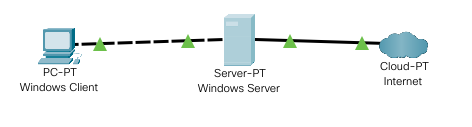
\includegraphics{net.png}
    \end{center}

    \textbf{пункт 6}
    \begin{center}
        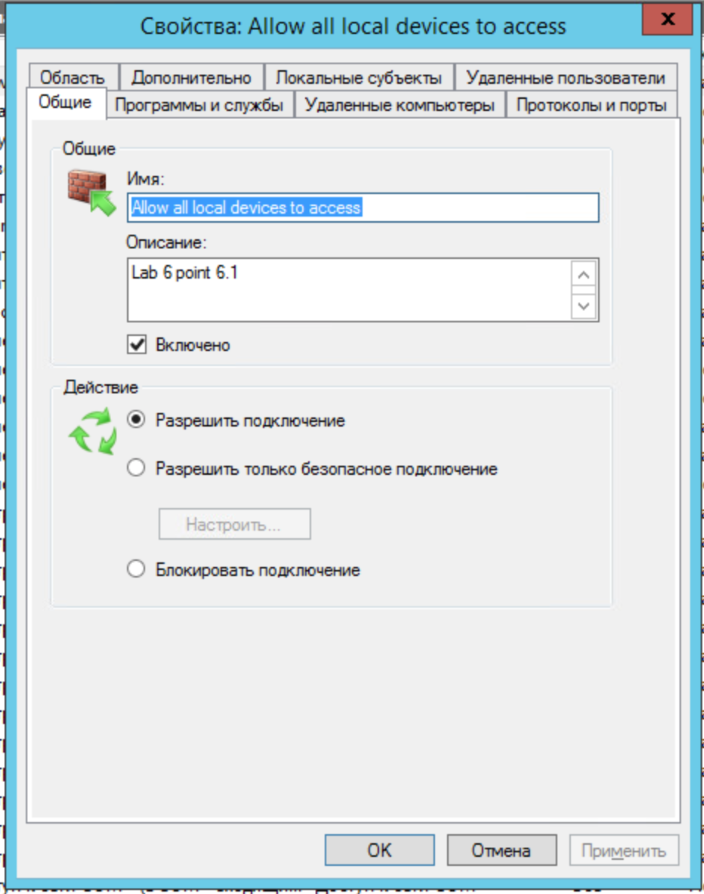
\includegraphics[scale=0.7]{6.1.1.png}
    \end{center}
    \begin{center}
        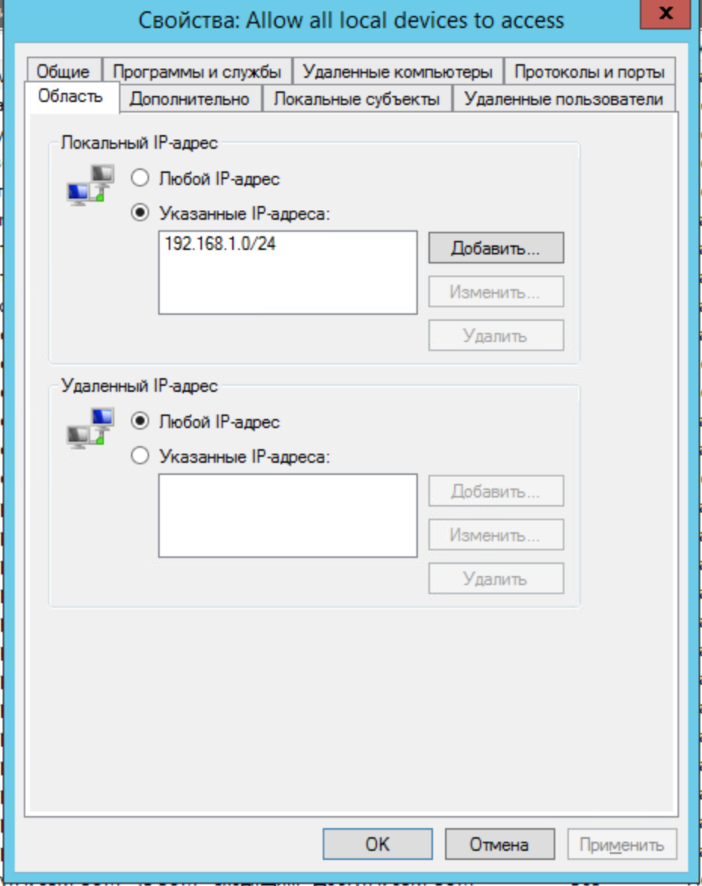
\includegraphics[scale=0.7]{6.1.2.png}
    \end{center}

    \begin{center}
        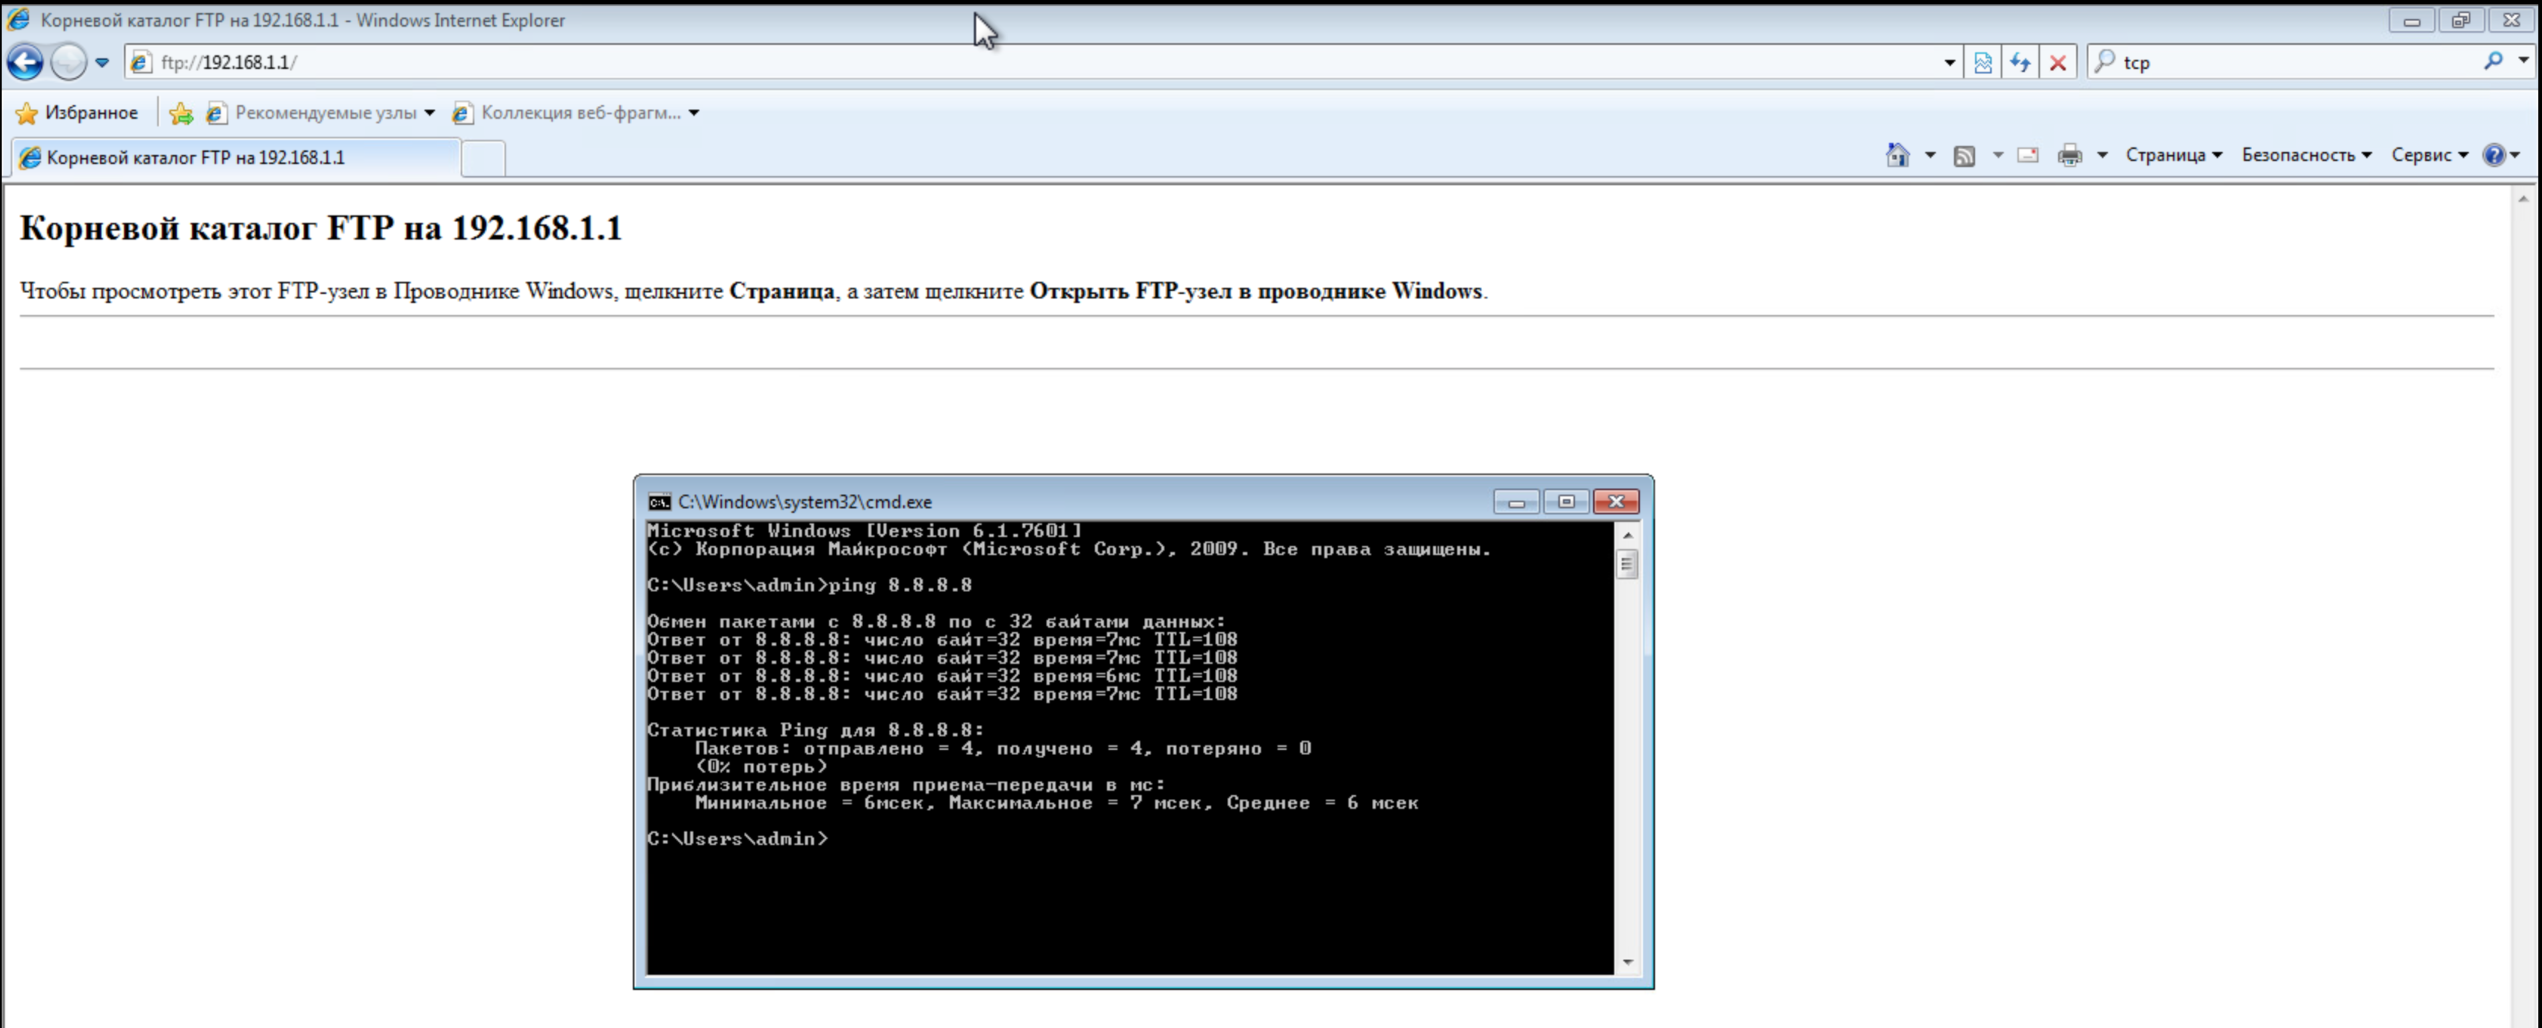
\includegraphics[scale=0.4]{6.1.3.png}
    \end{center}

    \begin{center}
        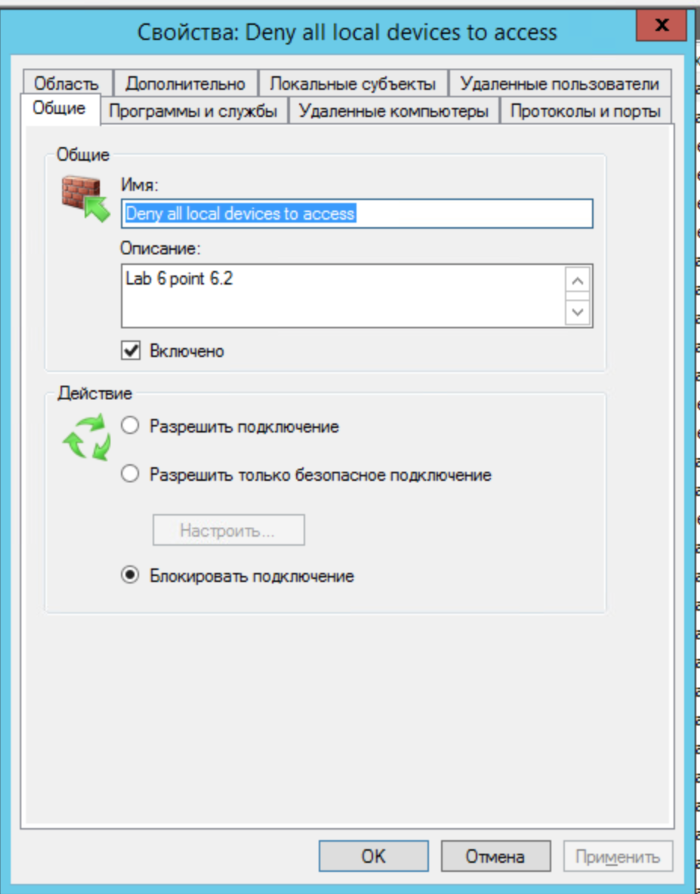
\includegraphics[scale=0.7]{6.2.1.png}
    \end{center}

    \begin{center}
        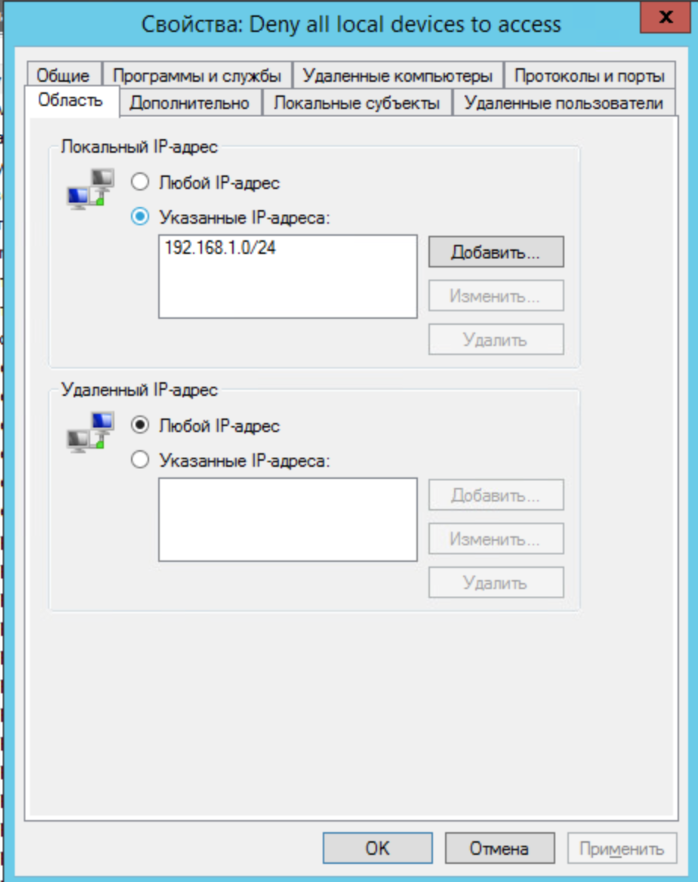
\includegraphics[scale=0.7]{6.2.2.png}
    \end{center}

    \begin{center}
        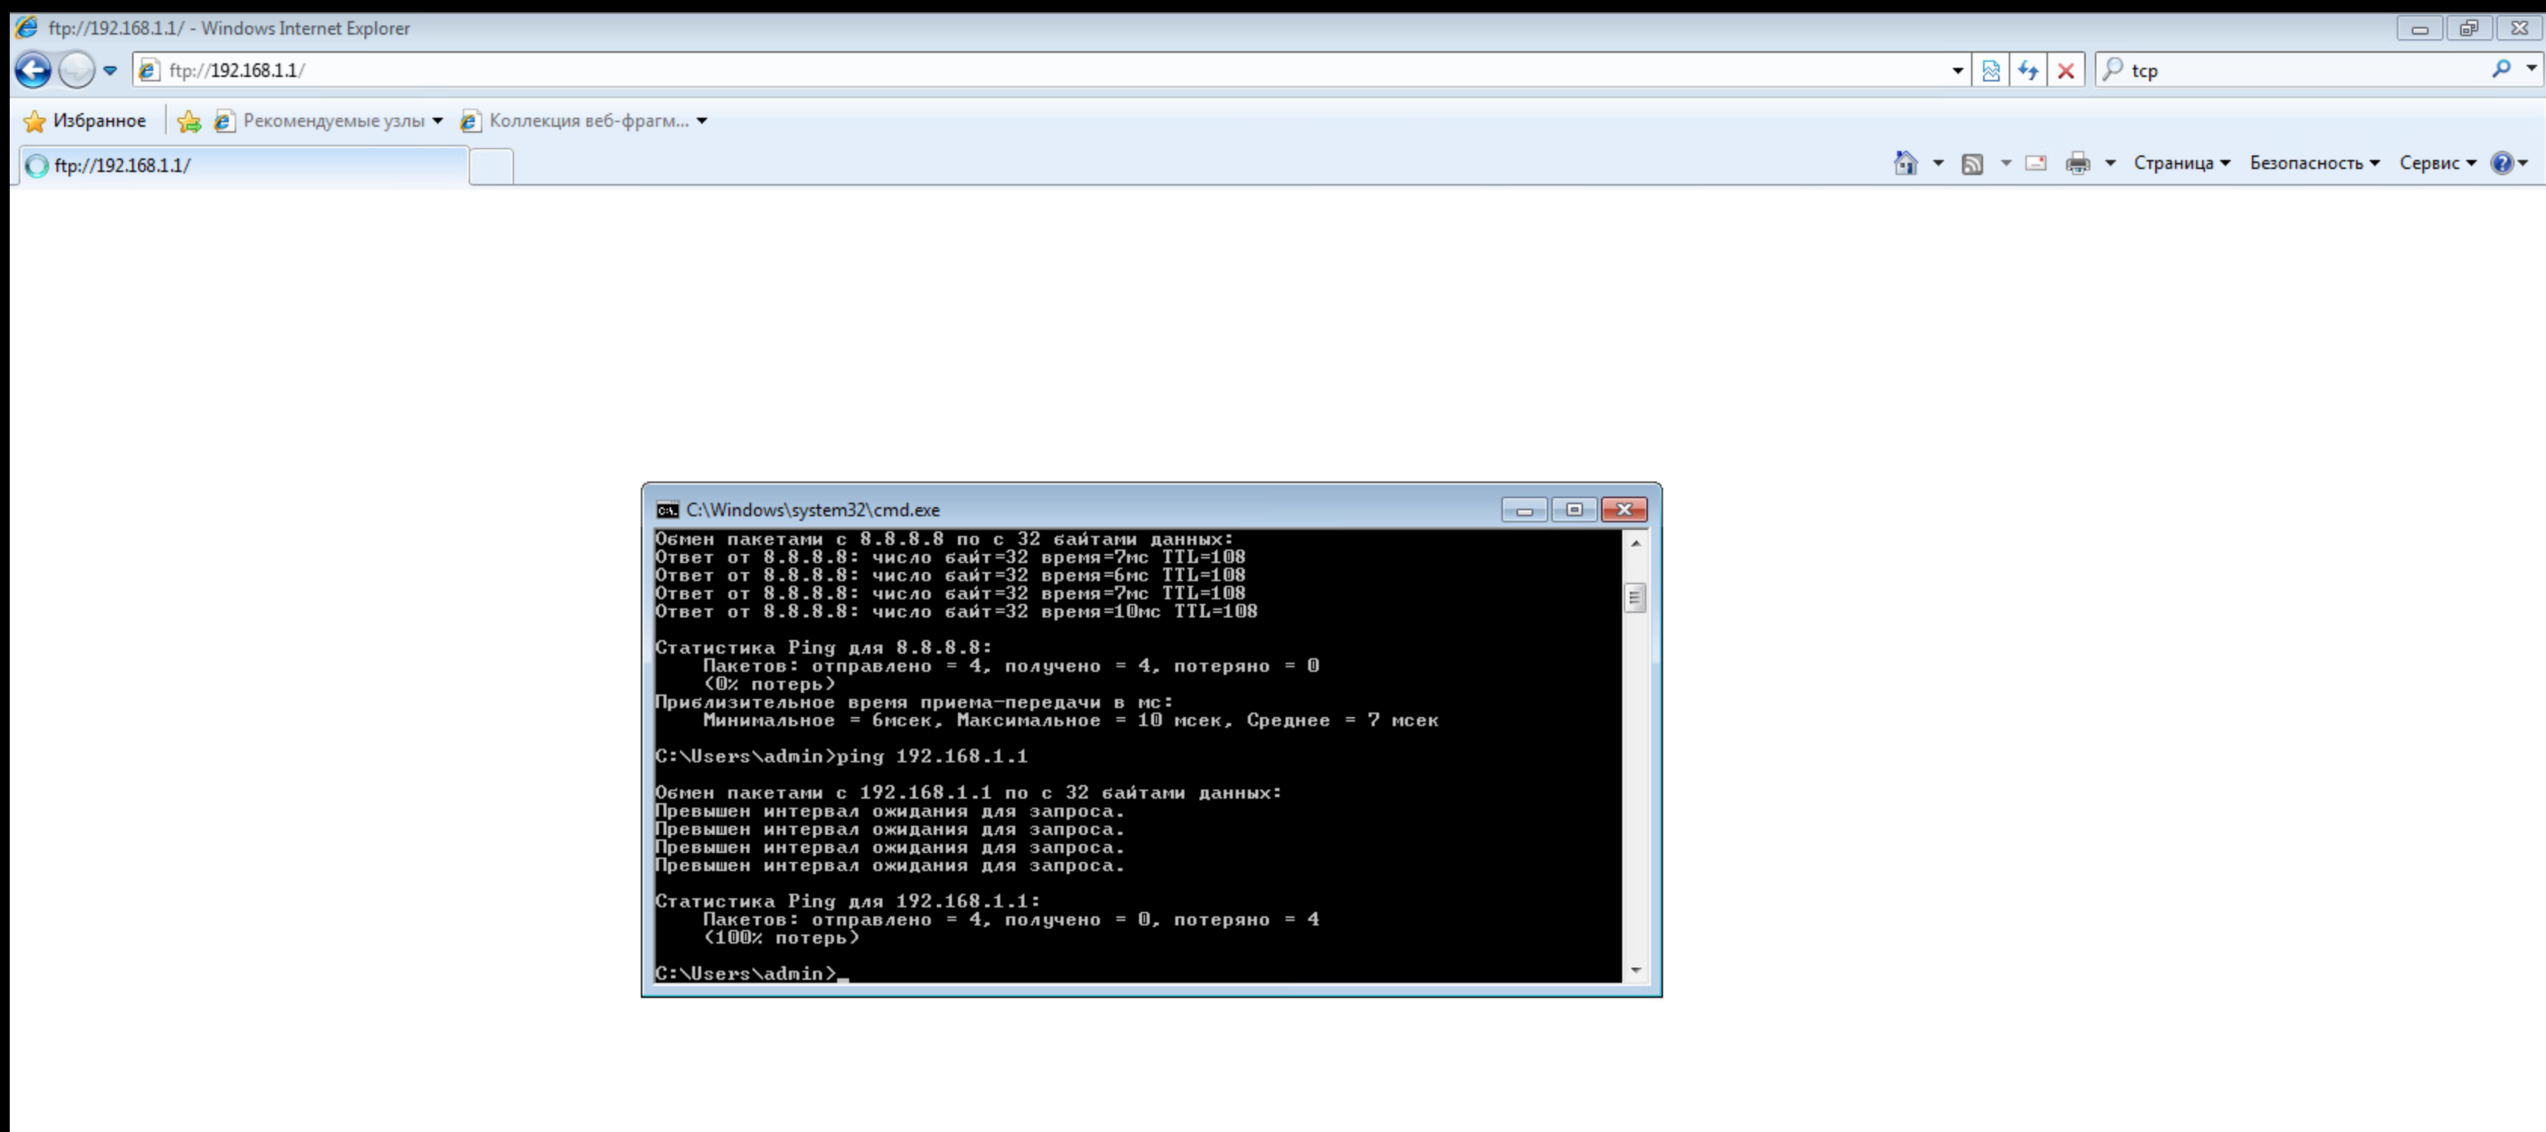
\includegraphics[scale=0.4]{6.2.3.png}
    \end{center}

    \newpage
    \textbf{пункт 7}
    \begin{center}
        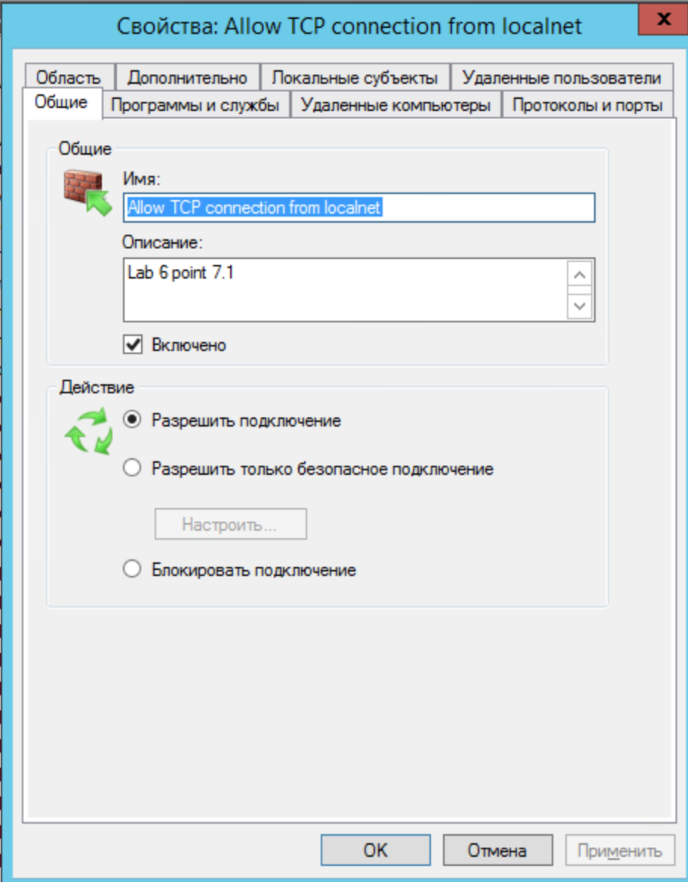
\includegraphics[scale=0.7]{7.1.1.png}
    \end{center}

    \begin{center}
        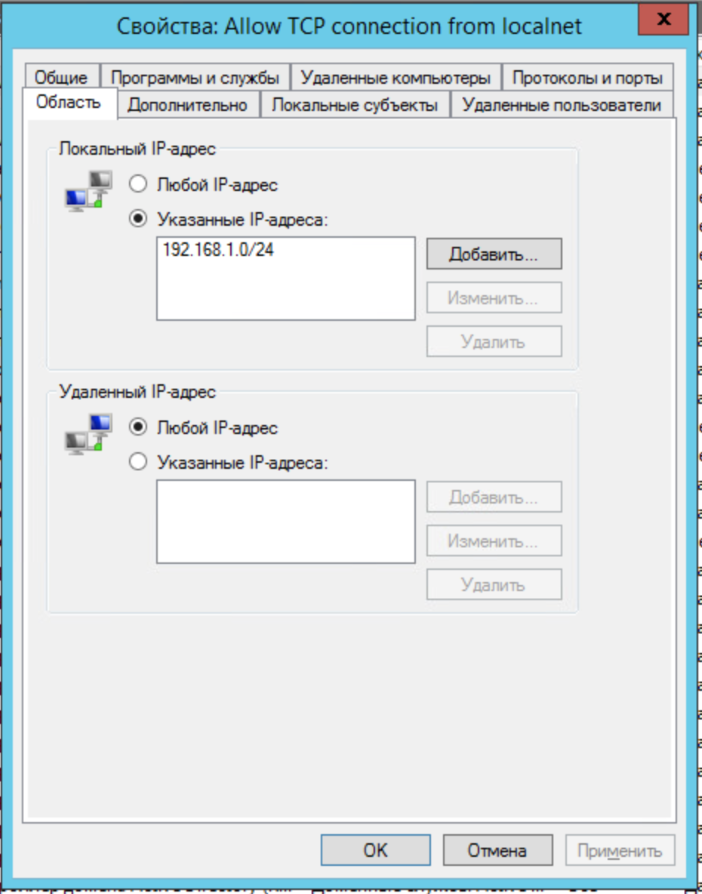
\includegraphics[scale=0.7]{7.1.2.png}
    \end{center}

    \begin{center}
        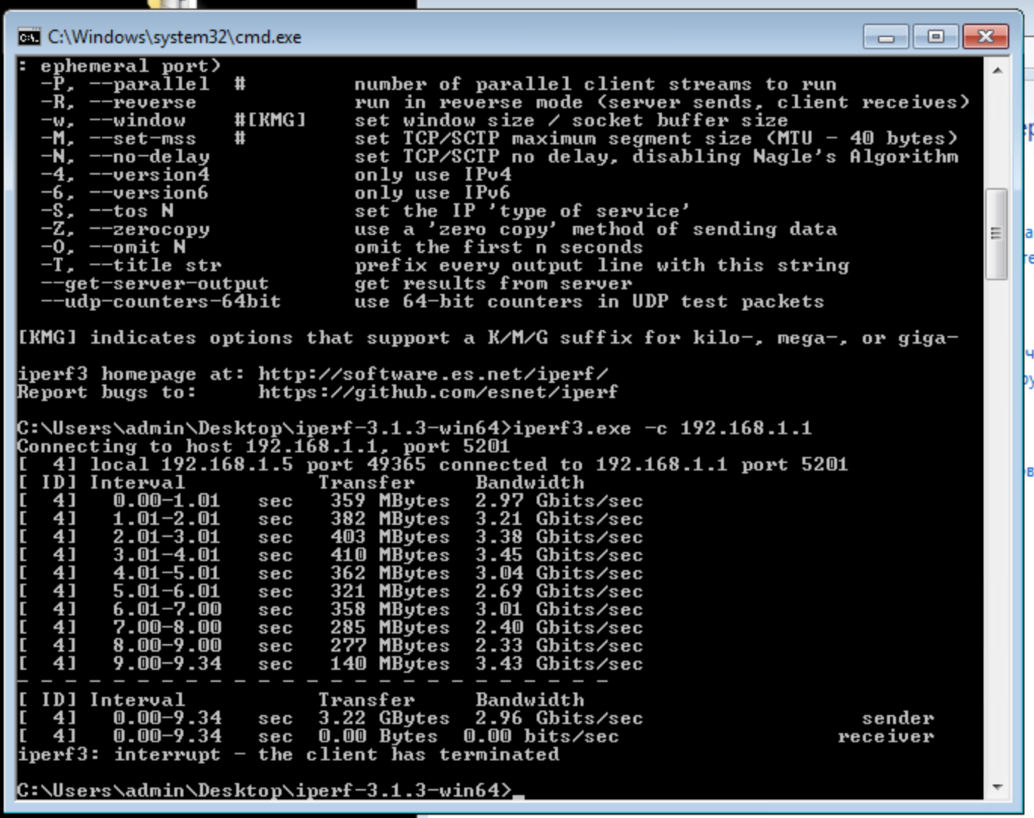
\includegraphics[scale=0.8]{7.1.3.png}
    \end{center}

    \begin{center}
        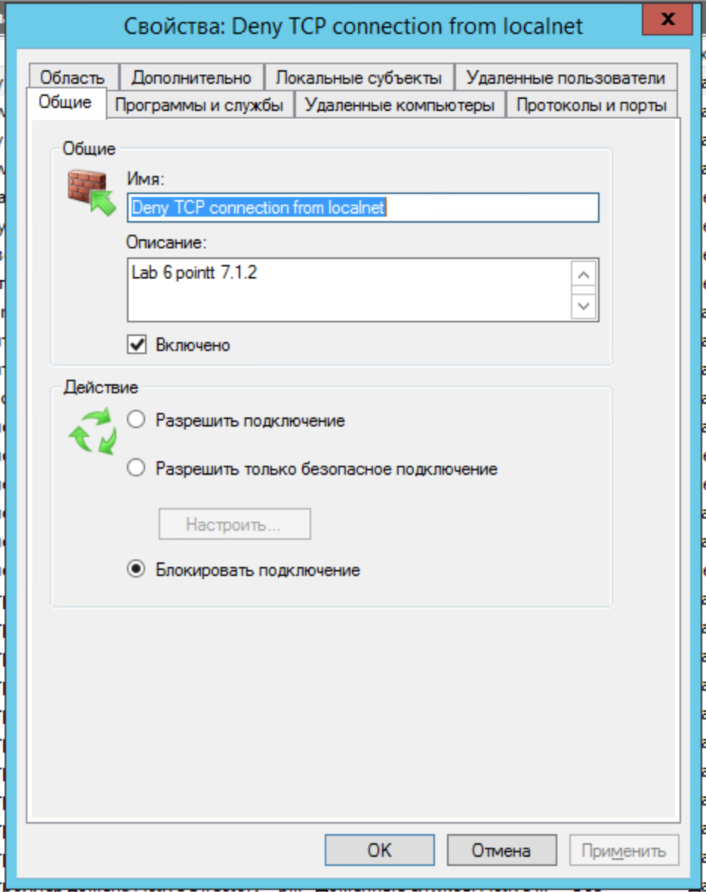
\includegraphics[scale=0.7]{7.2.1.png}
    \end{center}

    \begin{center}
        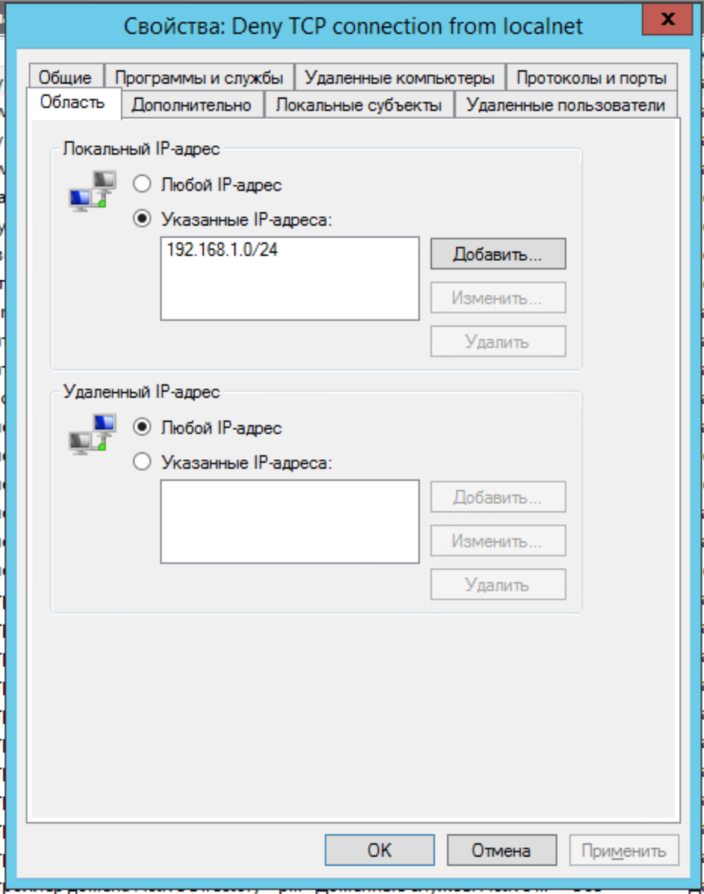
\includegraphics[scale=0.7]{7.2.2.png}
    \end{center}

    \begin{center}
        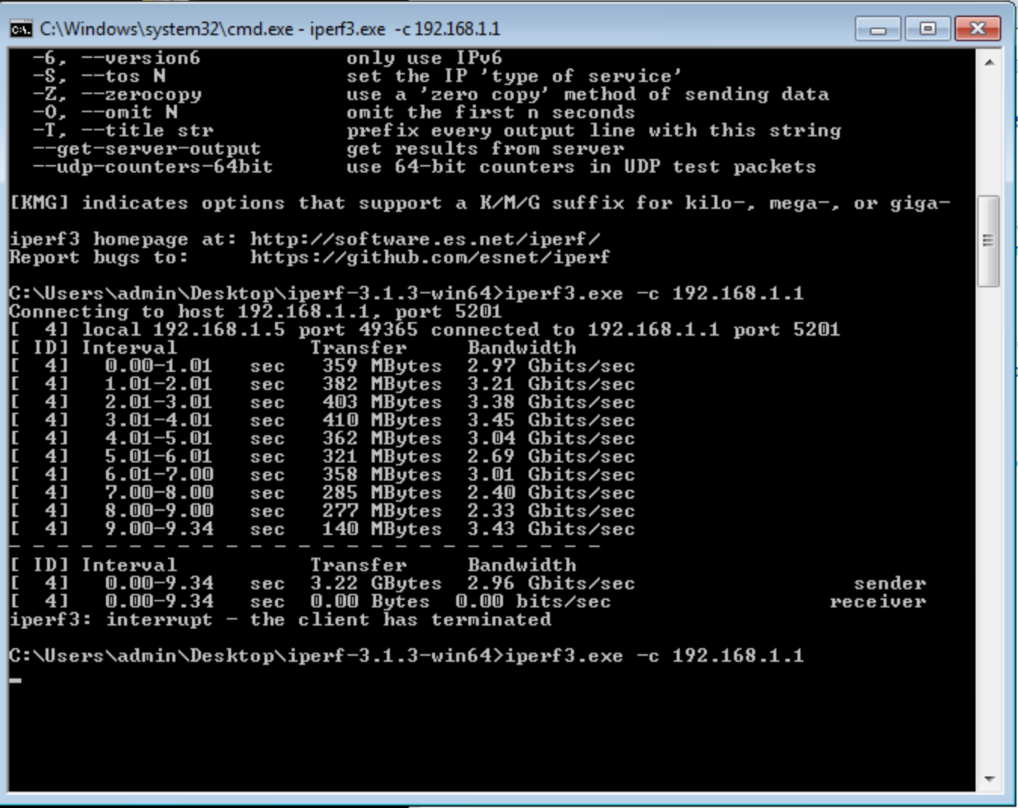
\includegraphics[scale=0.8]{7.2.3.png}
    \end{center}

    \begin{center}
        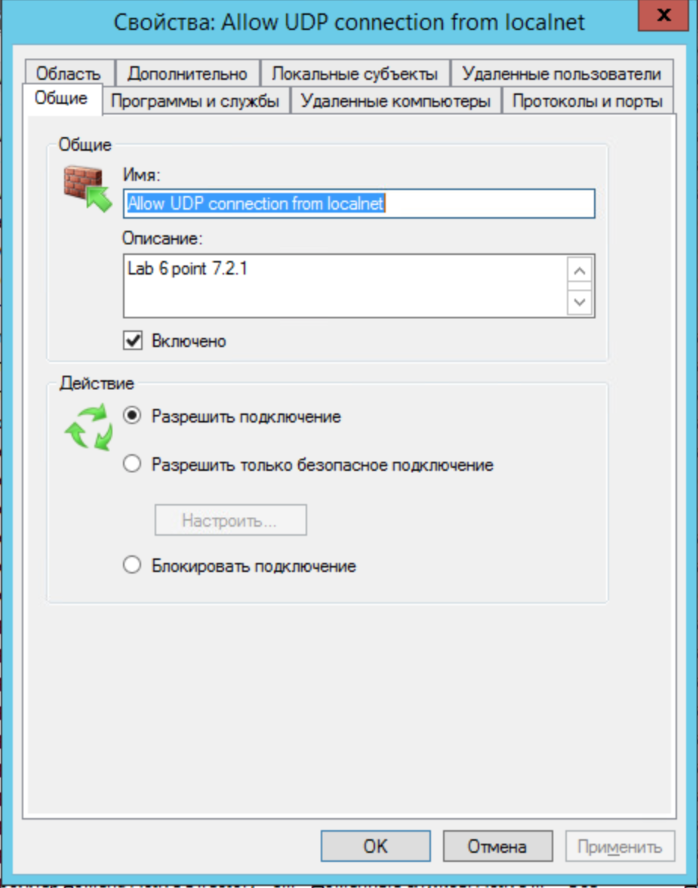
\includegraphics[scale=0.7]{7.3.1.png}
    \end{center}

    \begin{center}
        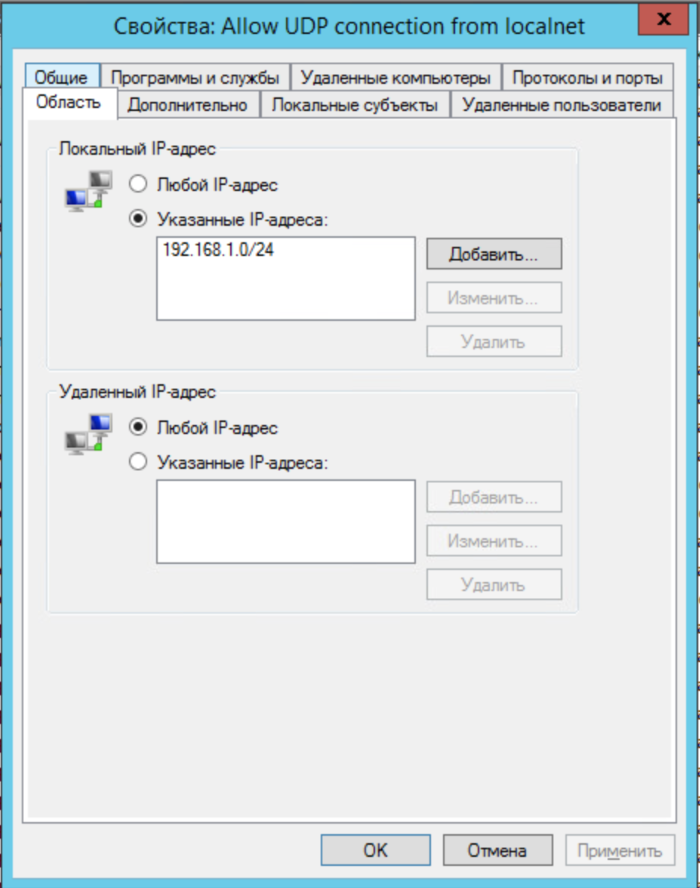
\includegraphics[scale=0.7]{7.3.2.png}
    \end{center}

    \begin{center}
        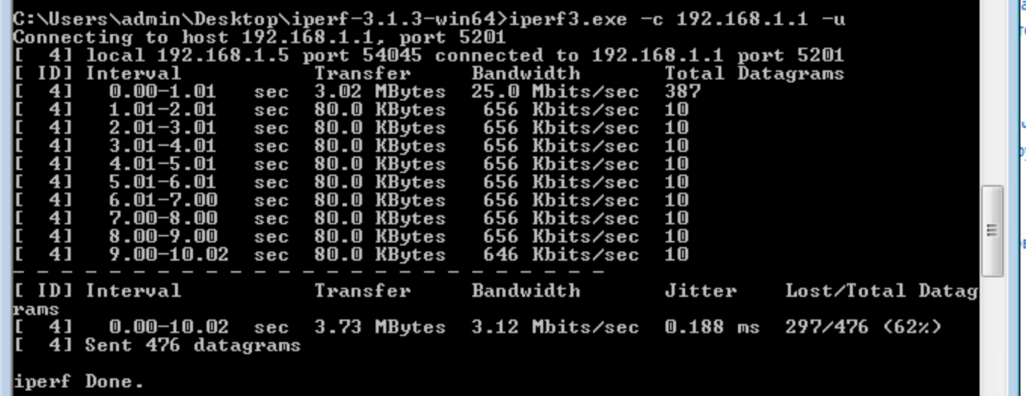
\includegraphics[scale=0.8]{7.3.3.png}
    \end{center}

    \begin{center}
        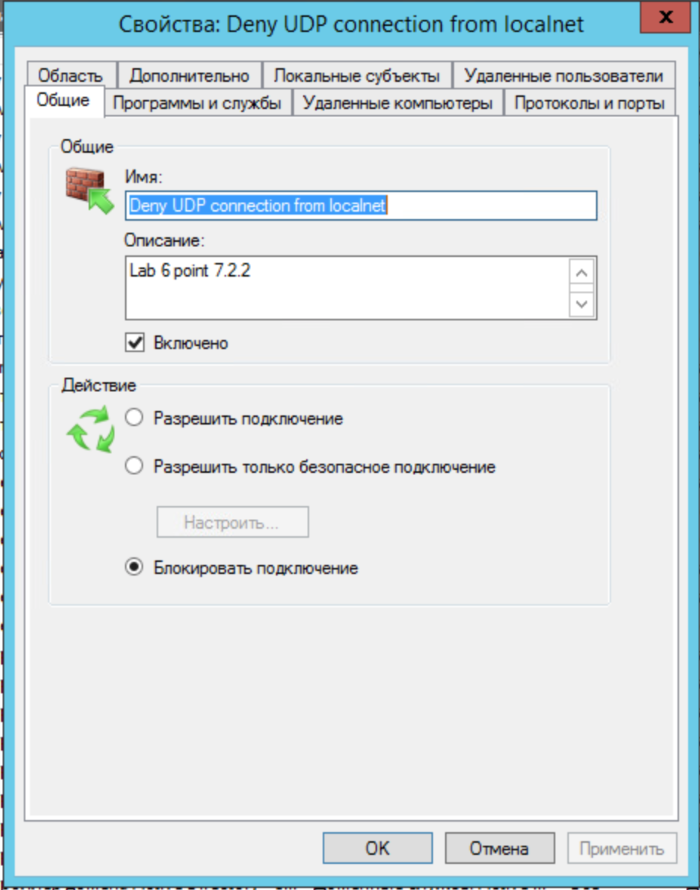
\includegraphics[scale=0.7]{7.4.1.png}
    \end{center}

    \begin{center}
        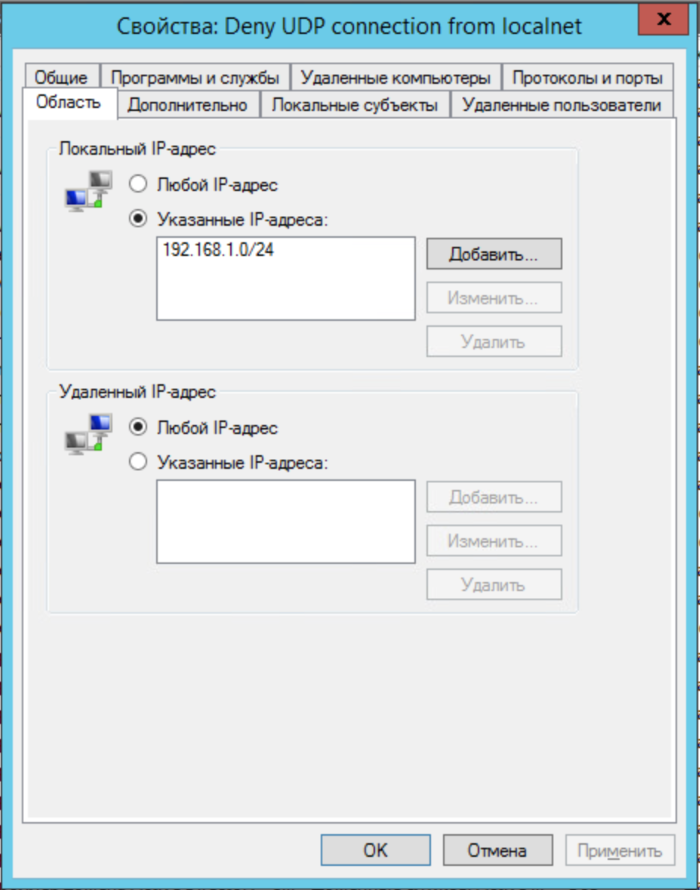
\includegraphics[scale=0.7]{7.4.2.png}
    \end{center}

    \begin{center}
        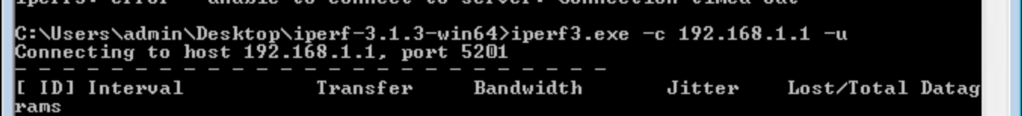
\includegraphics[scale=0.8]{7.4.3.png}
    \end{center}

    \begin{center}
        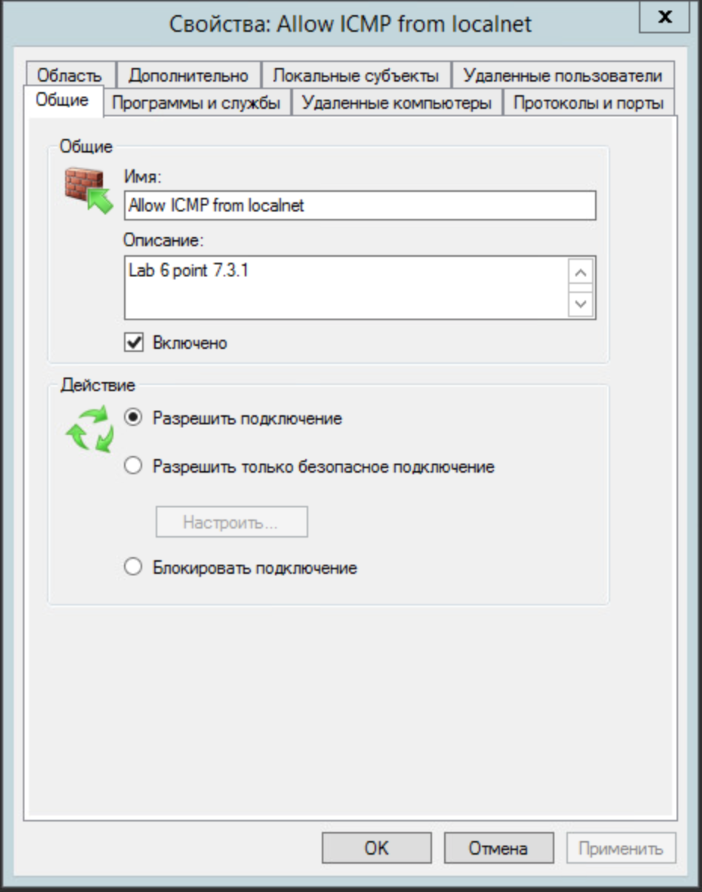
\includegraphics[scale=0.7]{7.5.1.png}
    \end{center}

    \begin{center}
        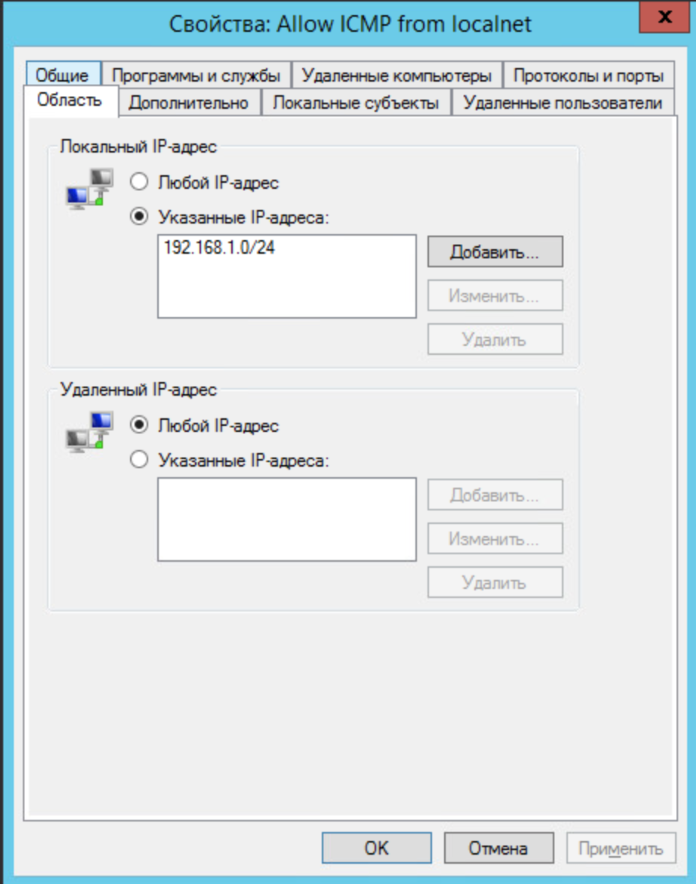
\includegraphics[scale=0.7]{7.5.2.png}
    \end{center}

    \begin{center}
        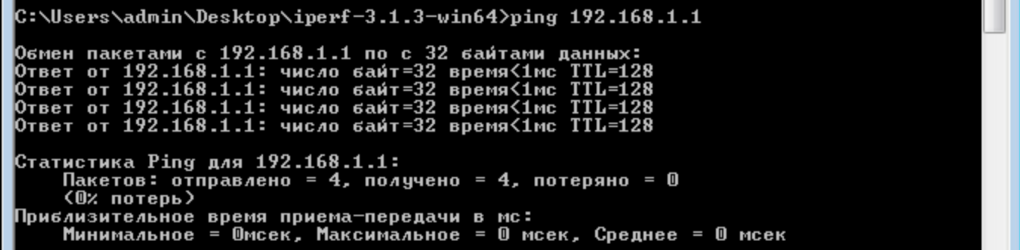
\includegraphics[scale=0.8]{7.5.3.png}
    \end{center}

    \begin{center}
        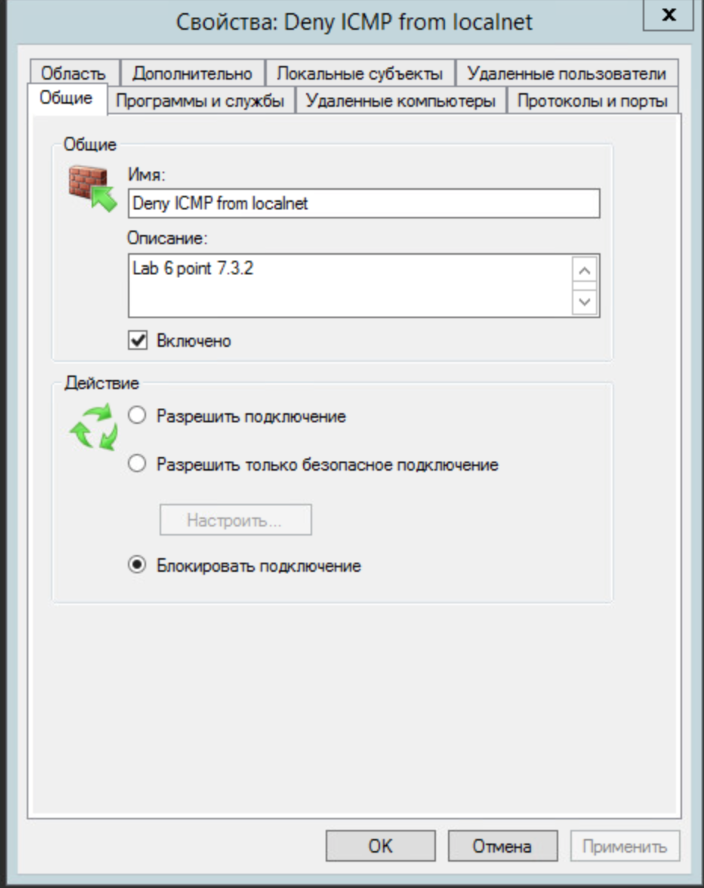
\includegraphics[scale=0.7]{7.6.1.png}
    \end{center}

    \begin{center}
        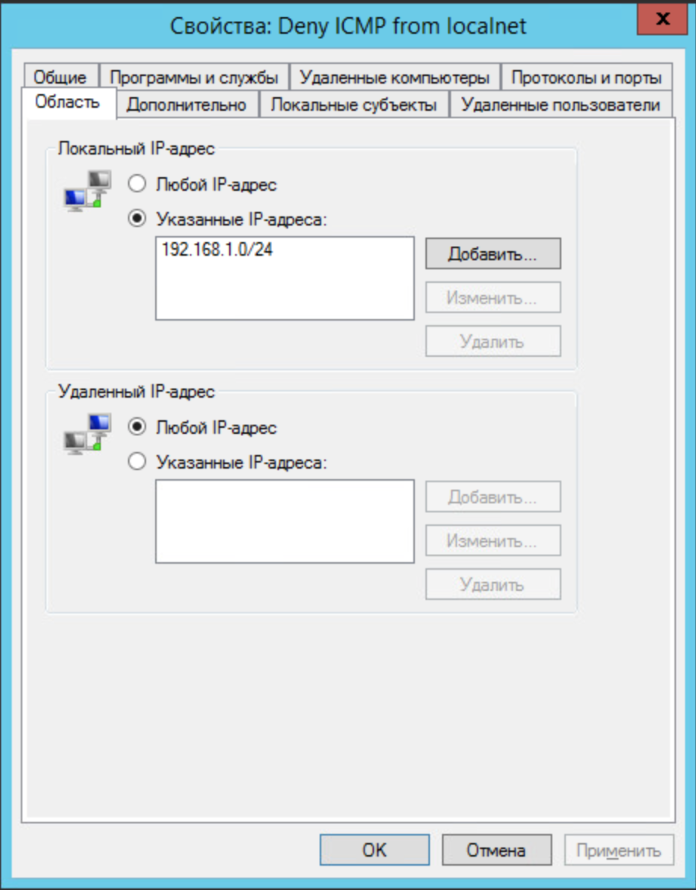
\includegraphics[scale=0.7]{7.6.2.png}
    \end{center}

    \begin{center}
        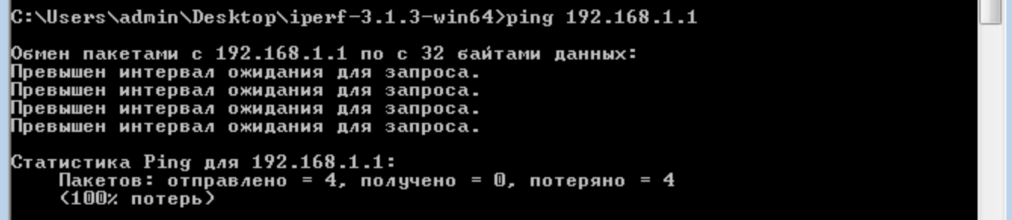
\includegraphics[scale=0.8]{7.6.3.png}
    \end{center}

    \newpage
    \textbf{пункт 8}
    \begin{center}
        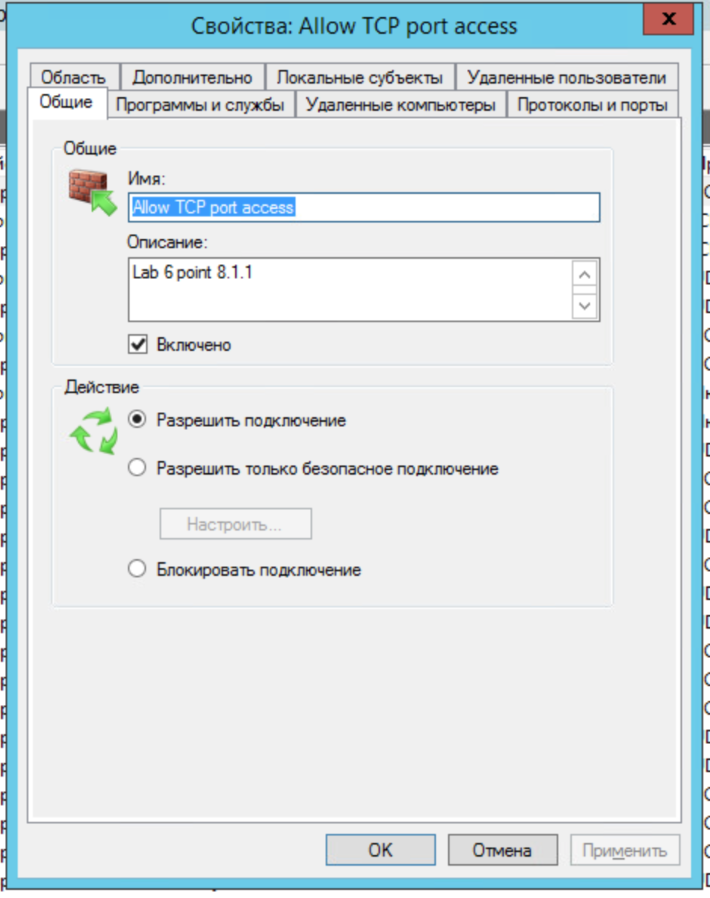
\includegraphics[scale=0.7]{8.1.1.png}
    \end{center}

    \begin{center}
        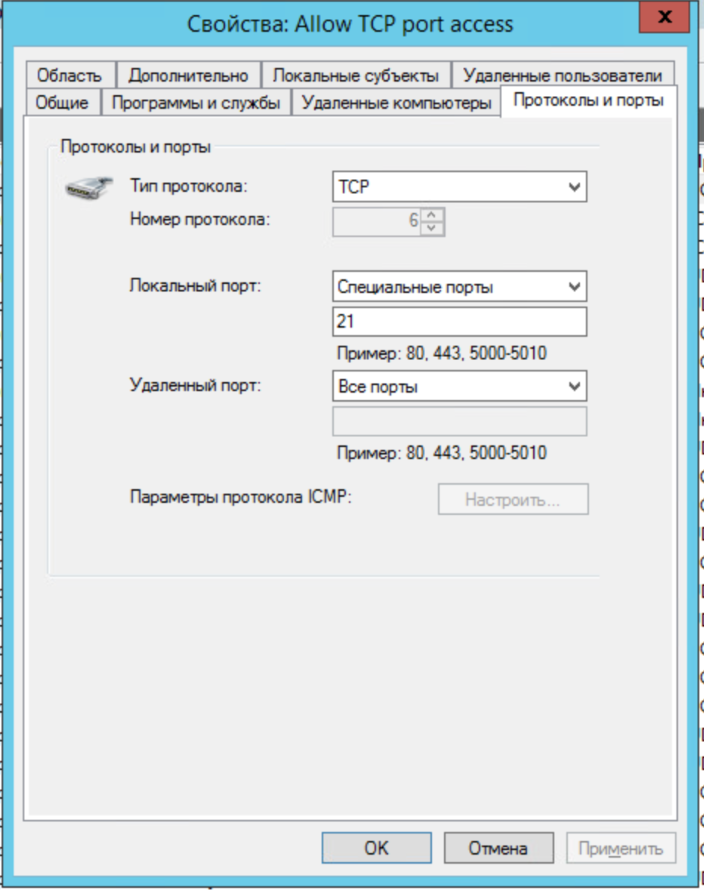
\includegraphics[scale=0.7]{8.1.2.png}
    \end{center}

    \begin{center}
        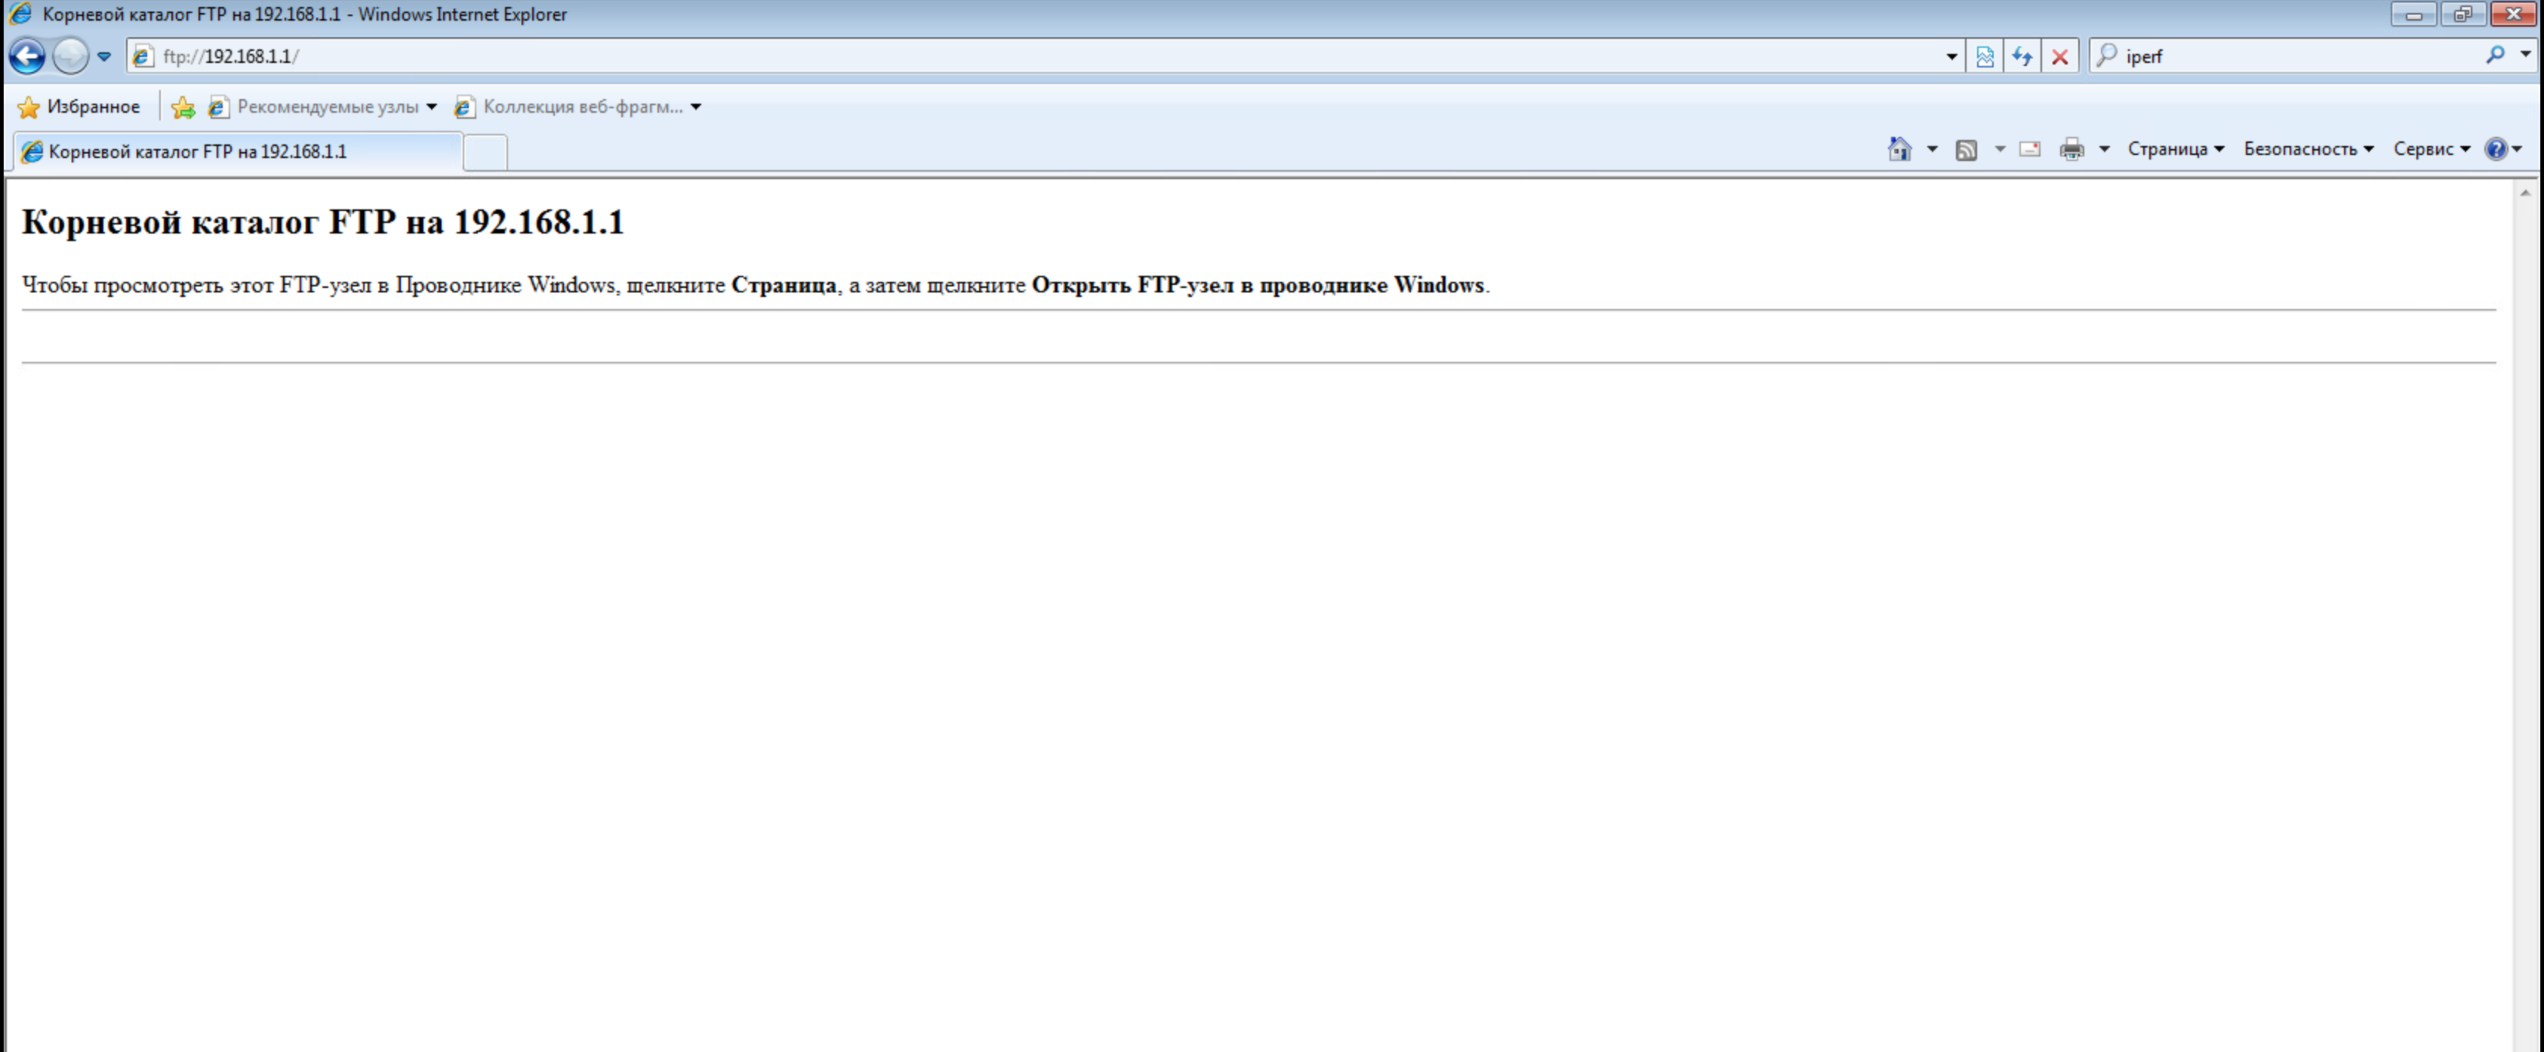
\includegraphics[scale=0.4]{8.1.3.png}
    \end{center}

    \begin{center}
        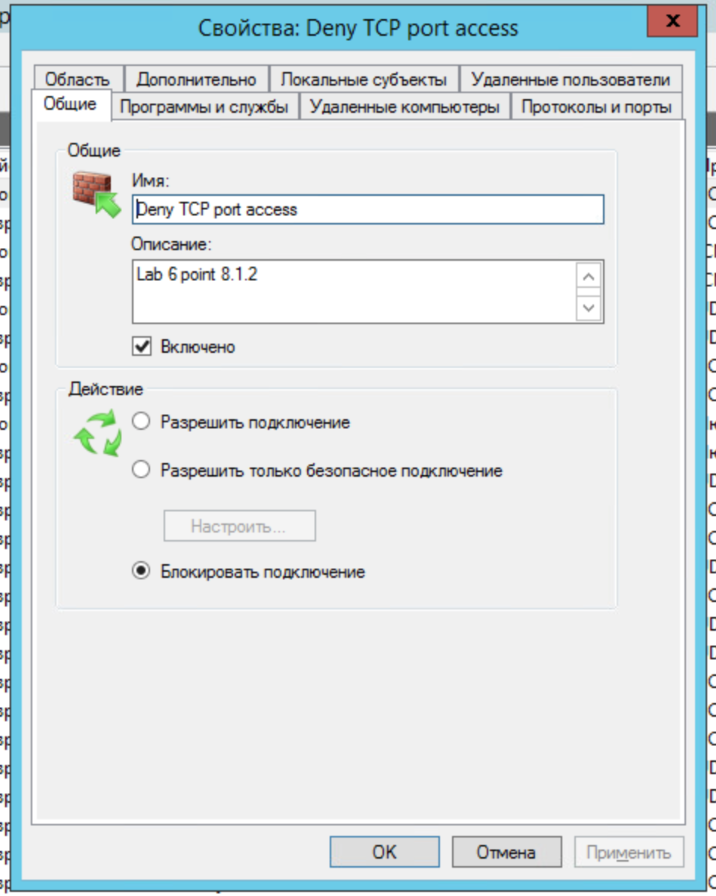
\includegraphics[scale=0.7]{8.2.1.png}
    \end{center}

    \begin{center}
        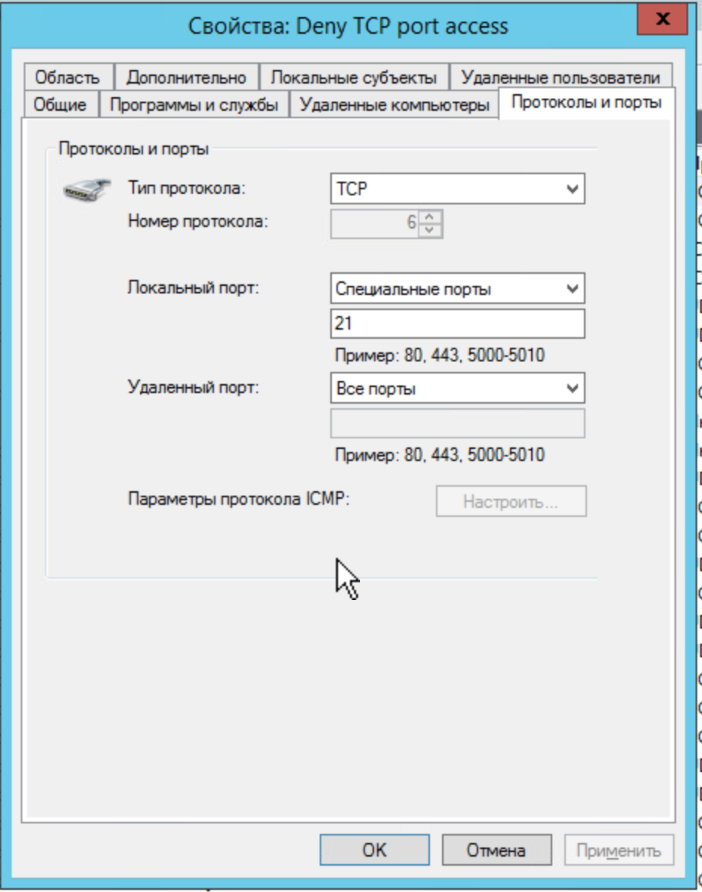
\includegraphics[scale=0.7]{8.2.2.png}
    \end{center}

    \begin{center}
        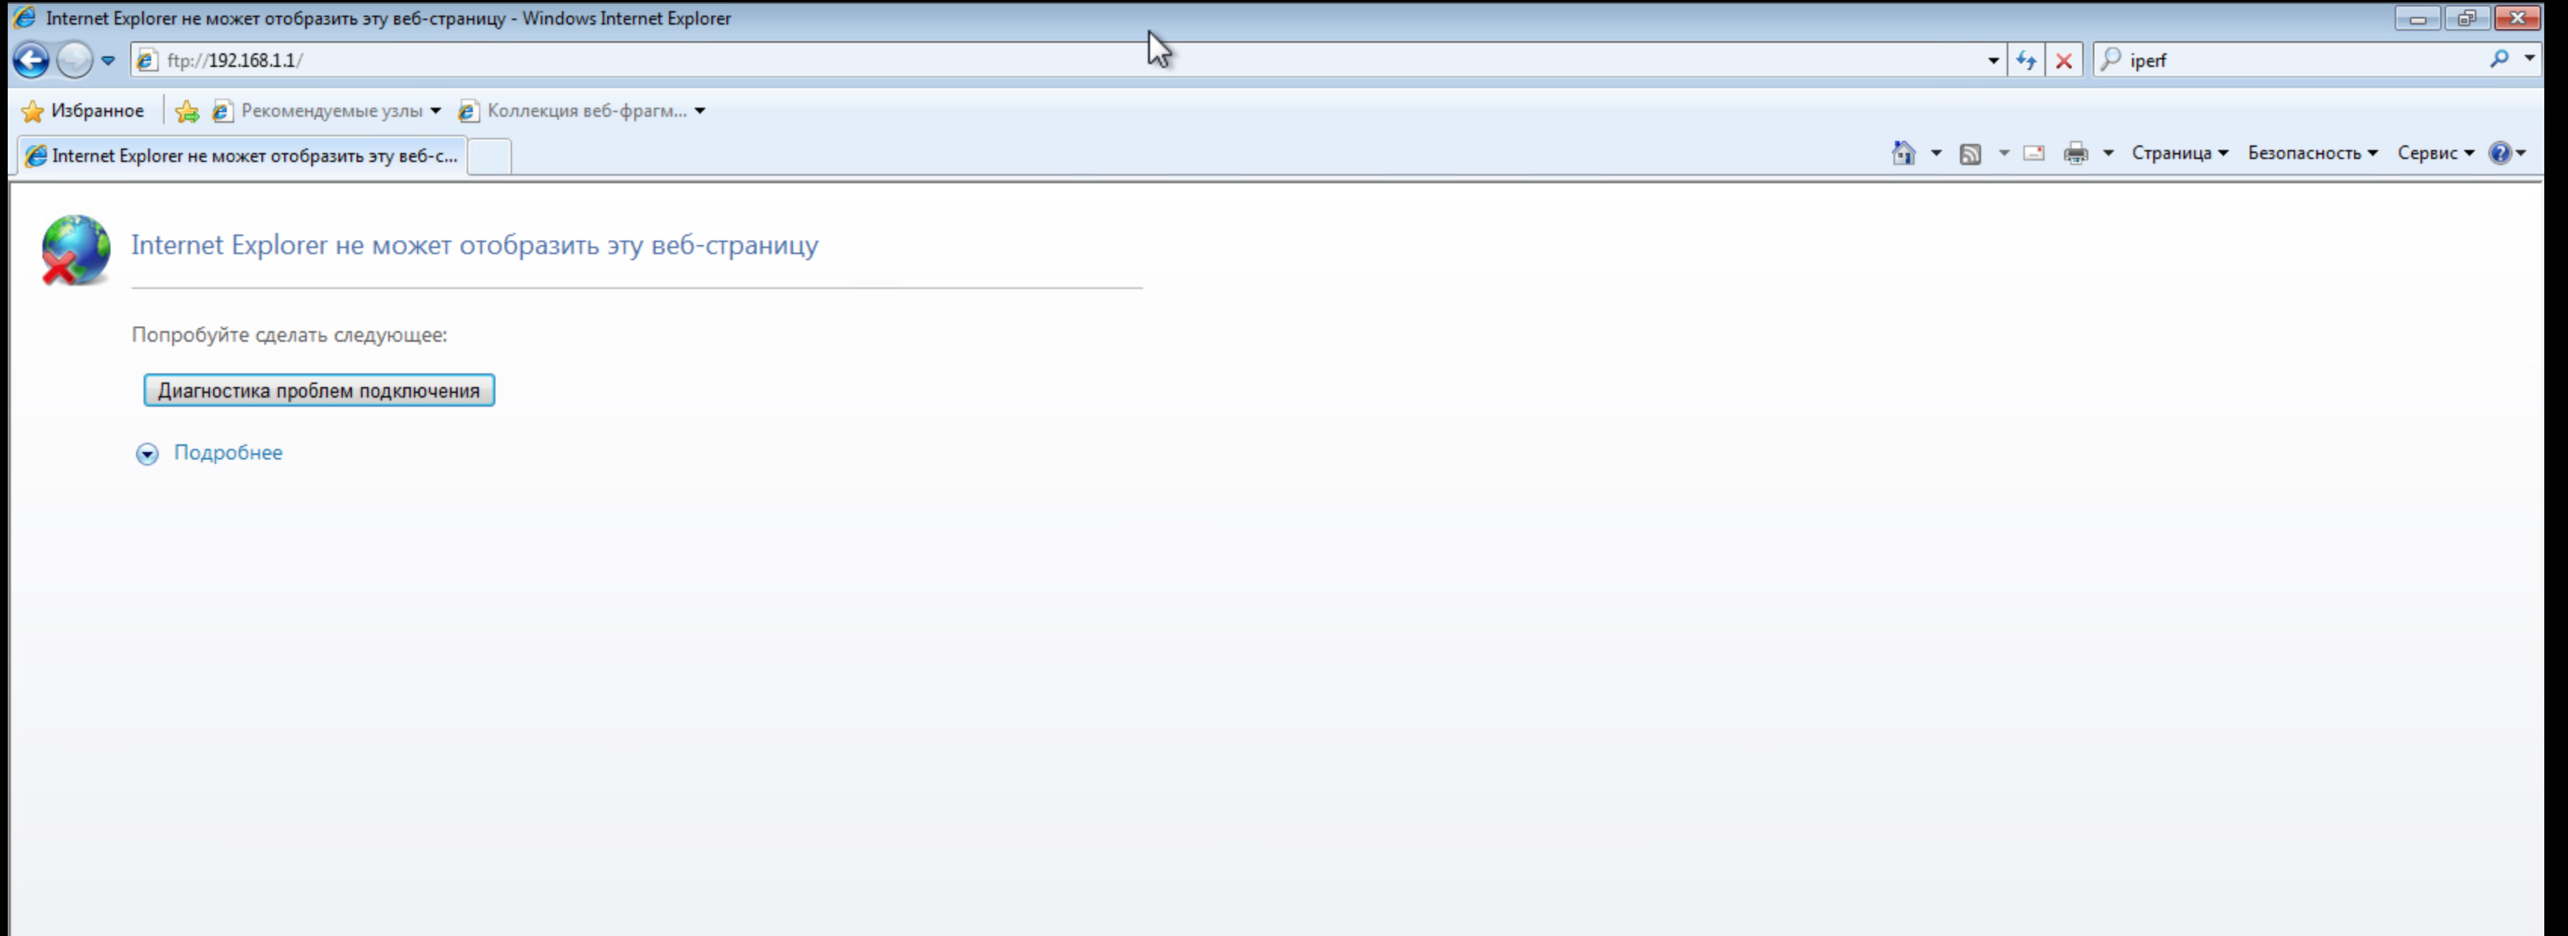
\includegraphics[scale=0.38]{8.2.3.png}
    \end{center}

    \begin{center}
        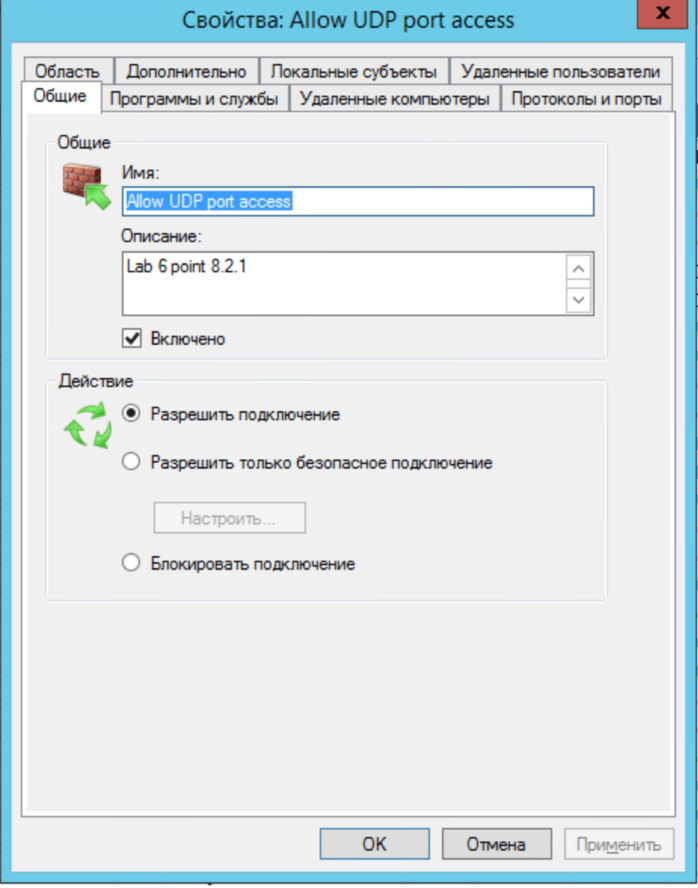
\includegraphics[scale=0.7]{8.3.1.png}
    \end{center}

    \begin{center}
        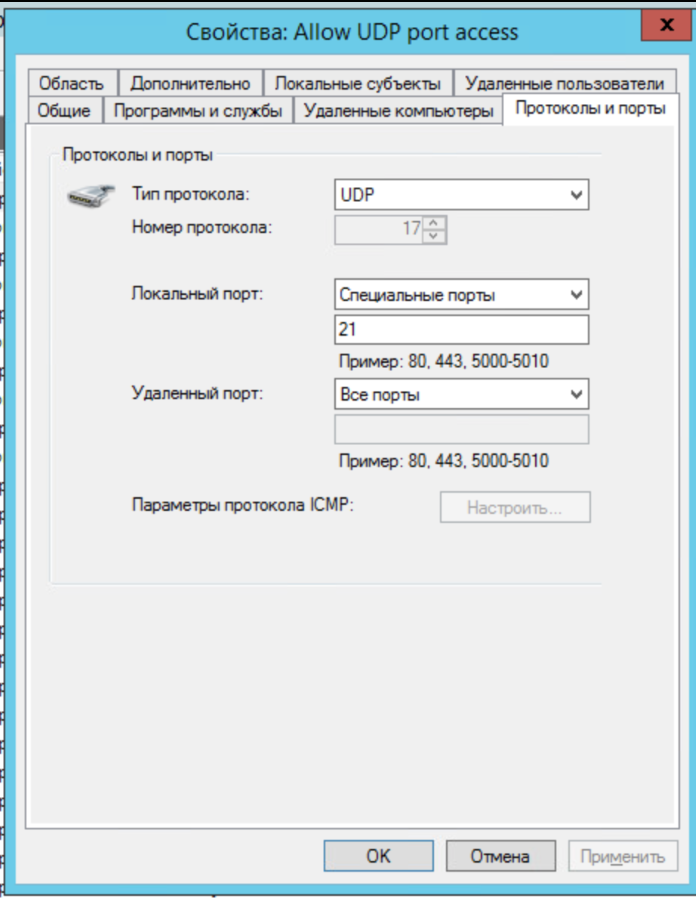
\includegraphics[scale=0.7]{8.3.2.png}
    \end{center}

    \begin{center}
        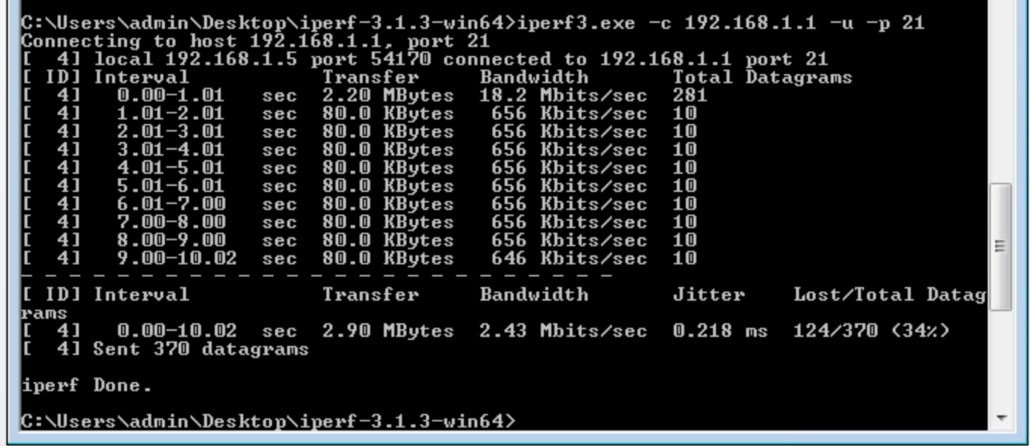
\includegraphics[scale=0.8]{8.3.3.png}
    \end{center}

    \begin{center}
        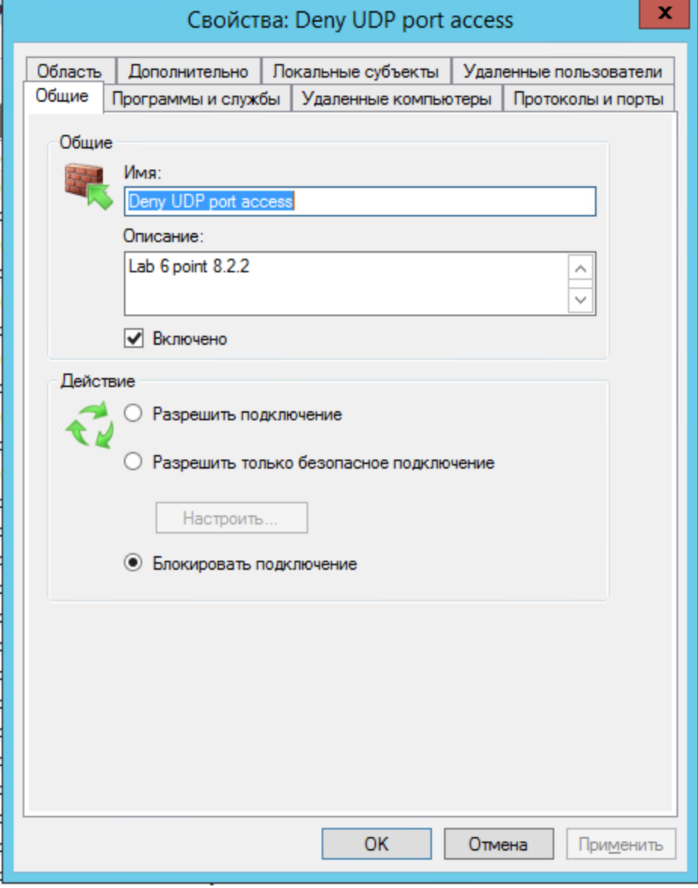
\includegraphics[scale=0.7]{8.4.1.png}
    \end{center}

    \begin{center}
        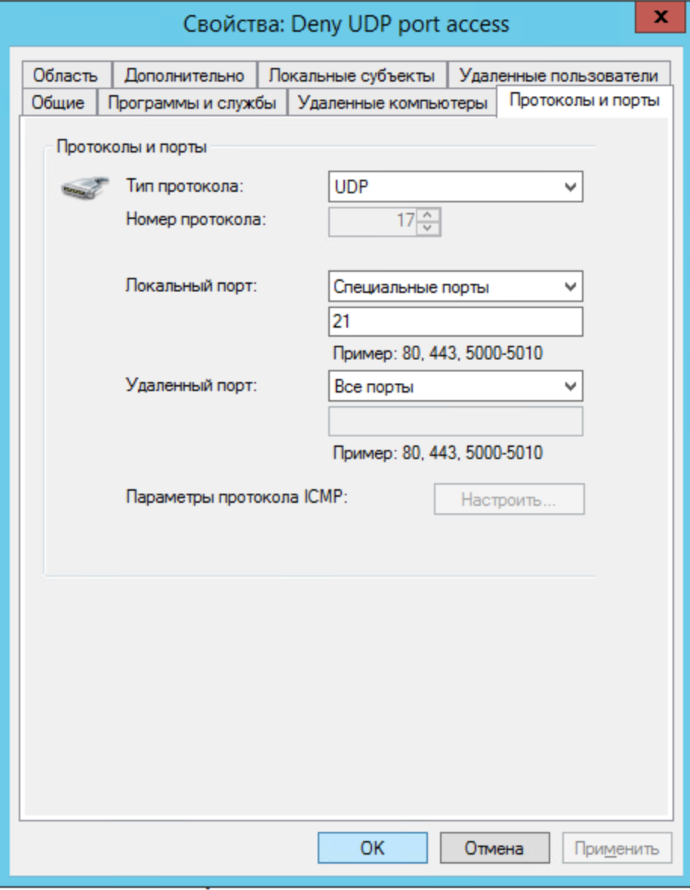
\includegraphics[scale=0.7]{8.4.2.png}
    \end{center}

    \begin{center}
        
\includegraphics[scale=0.8]{8.4.3.png}
    \end{center}

    \newpage
    \textbf{пункт 9}
    \begin{center}
        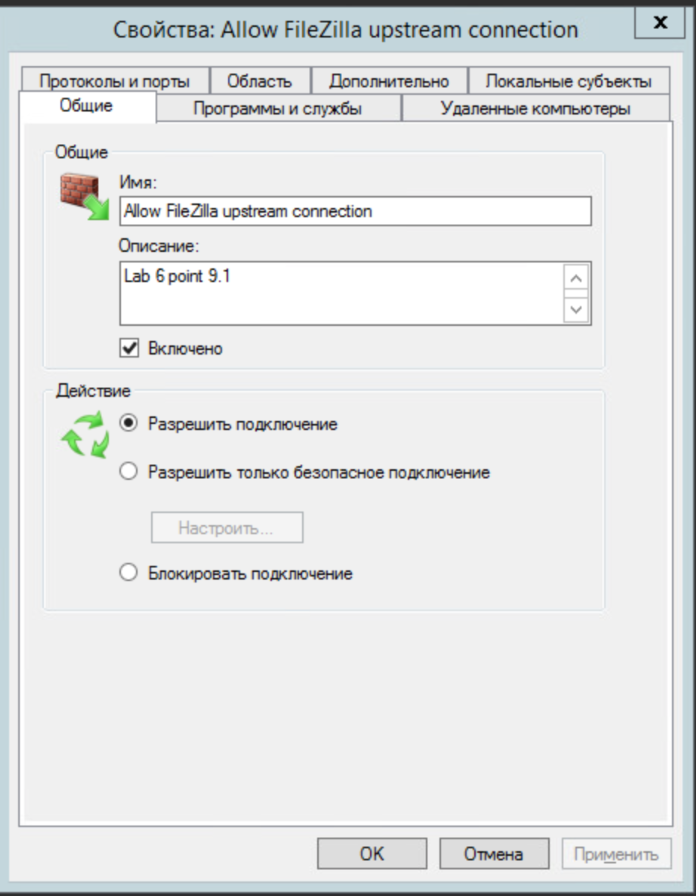
\includegraphics[scale=0.7]{9.1.1.png}
    \end{center}

    \begin{center}
        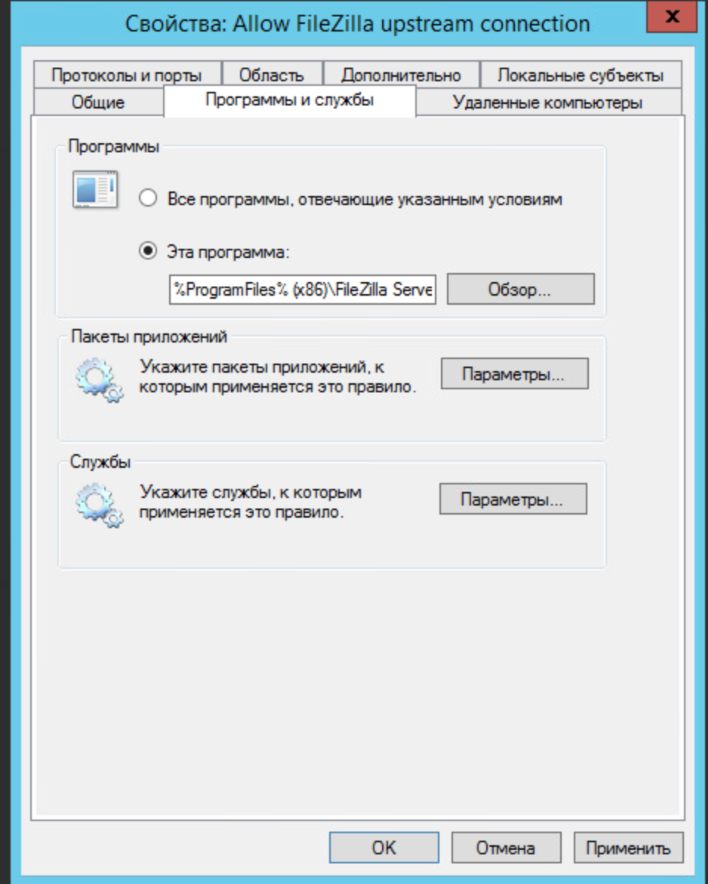
\includegraphics[scale=0.7]{9.1.2.png}
    \end{center}

    \begin{center}
        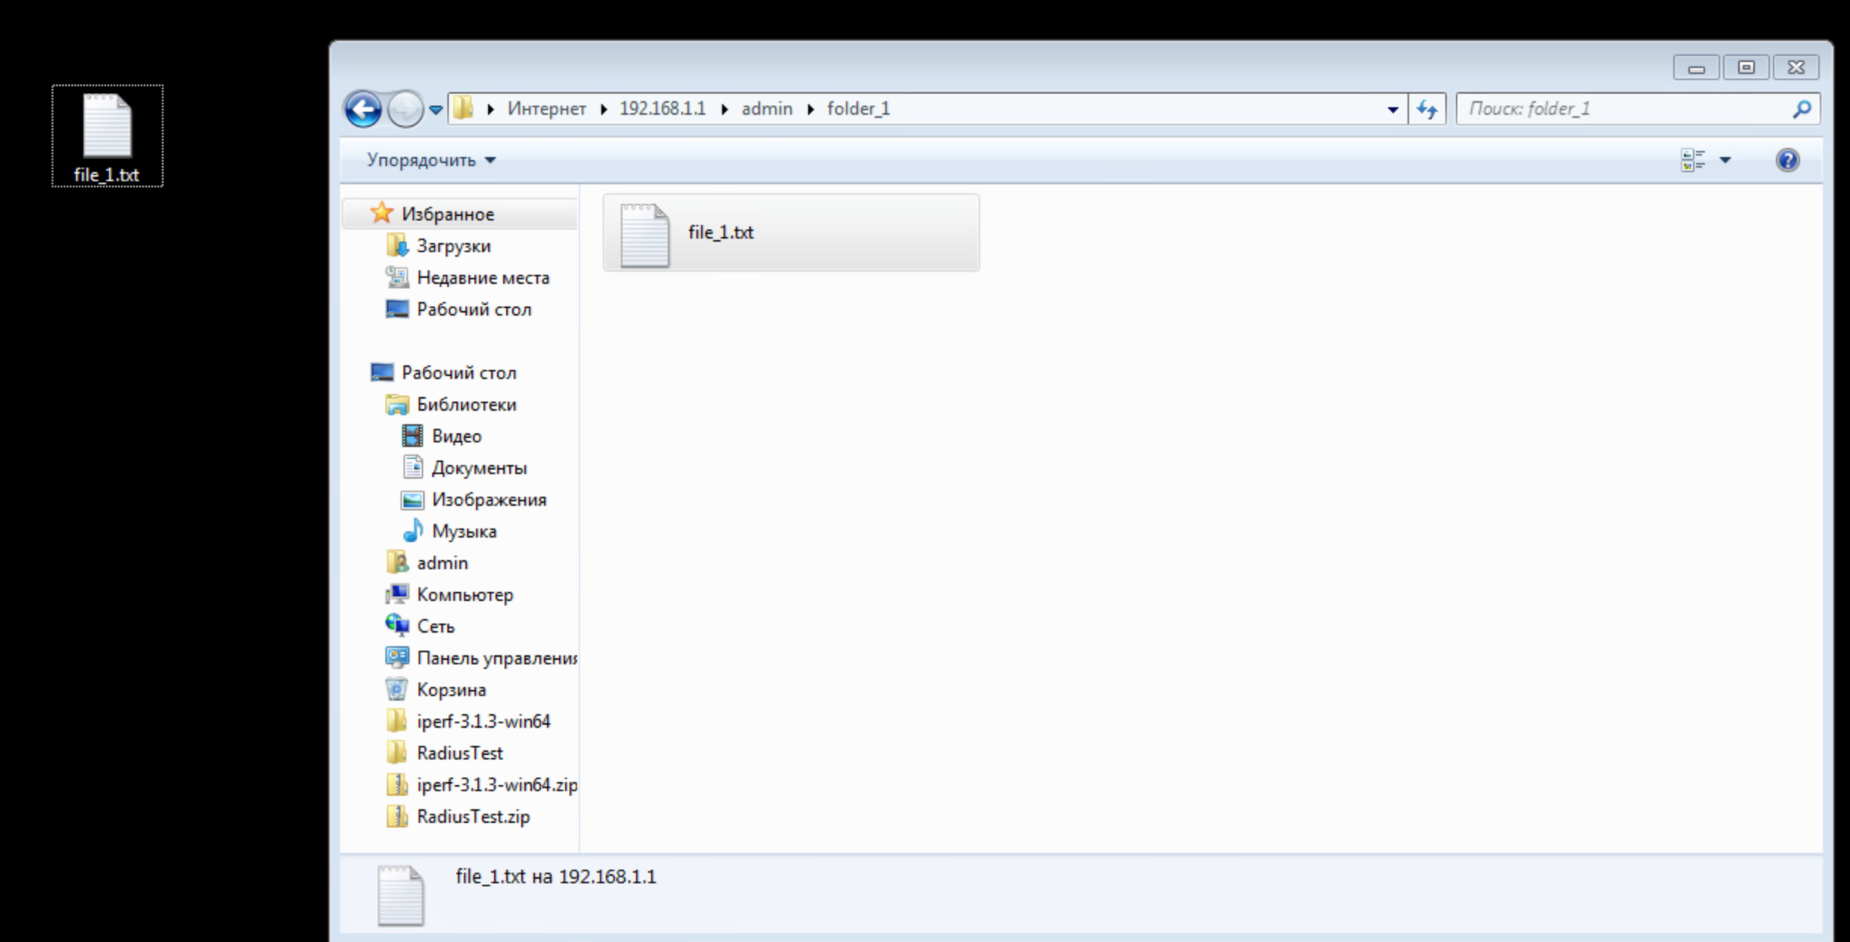
\includegraphics[scale=0.4]{9.1.3.png}
    \end{center}

    \begin{center}
        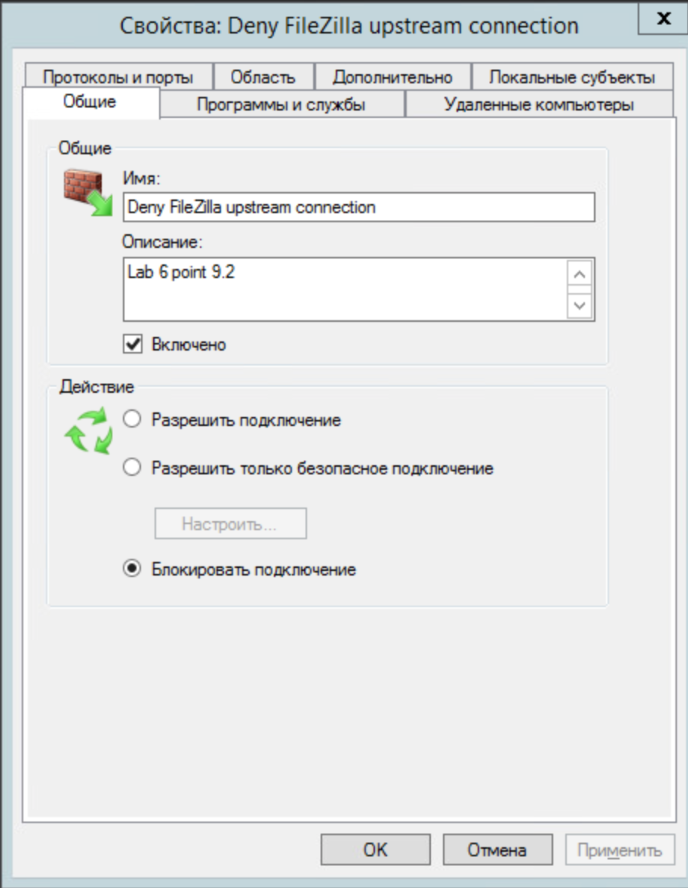
\includegraphics[scale=0.7]{9.2.1.png}
    \end{center}

    \begin{center}
        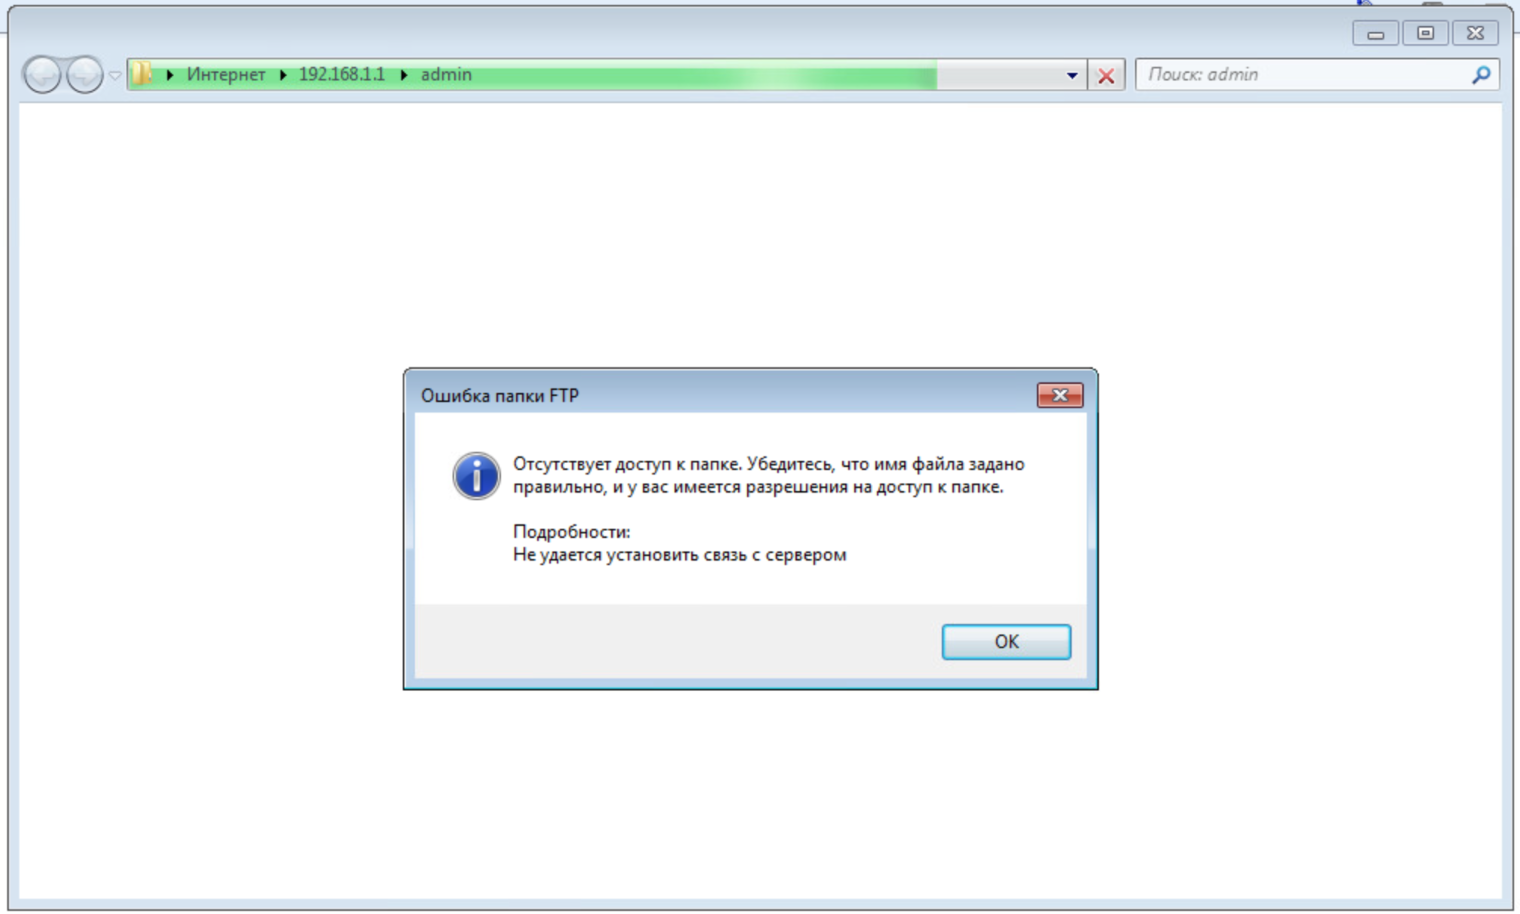
\includegraphics[scale=0.6]{9.2.2.png}
    \end{center}

    \textbf{Вывод:}

    В ходе данной лабораторной работы мы научились поднимать простейший ftp-server, создавать, настраивать и управлять правилами брандмауэра для разных протоколов, портов и приложений. Также мы провели проверку работоспособности данных правил.
  
\end{document}